% !TEX program = xelatex
\documentclass[UTF8,fontset=fandol,a4paper,11pt]{ctexart}
\usepackage[margin=21mm,top=23mm,bottom=22mm,headheight=16pt]{geometry}
\usepackage{amsmath,amssymb,mathtools,bm}
\usepackage{tikz}
\usetikzlibrary{arrows.meta,calc,angles,quotes,patterns}
\usepackage{xcolor,booktabs,array,longtable,enumitem,fancyhdr,needspace}
\usepackage[unicode,hidelinks]{hyperref}
\definecolor{ink}{HTML}{24343C}
\definecolor{accent}{HTML}{166A70}
\definecolor{muted}{HTML}{65747A}
\definecolor{rulegray}{HTML}{D4DDE0}
\definecolor{warm}{HTML}{966037}
\color{ink}
\setlength{\parindent}{2em}
\setlength{\parskip}{4pt}
\linespread{1.12}
\AtBeginDocument{\setlength{\abovedisplayskip}{6pt plus 2pt minus 1pt}
\setlength{\belowdisplayskip}{6pt plus 2pt minus 1pt}
\setlength{\abovedisplayshortskip}{0pt plus 1pt}
\setlength{\belowdisplayshortskip}{4pt plus 1pt}}
\setlist[enumerate]{label=(\arabic*),leftmargin=2.3em,itemsep=3pt,topsep=4pt}
\setlist[itemize]{leftmargin=2em,itemsep=2pt,topsep=4pt}
\allowdisplaybreaks[1]
\setlength{\emergencystretch}{2em}
\setcounter{secnumdepth}{0}
\providecommand{\tightlist}{\setlength{\itemsep}{0pt}\setlength{\parskip}{0pt}}
\ctexset{section={format=\Large\bfseries\color{accent},beforeskip=10pt,afterskip=9pt},
subsection={format=\normalsize\bfseries\color{accent},beforeskip=10pt,afterskip=4pt},
subsubsection={format=\normalsize\bfseries,beforeskip=8pt,afterskip=3pt}}
\pagestyle{fancy}
\fancyhf{}
\fancyhead[L]{\small\color{muted}物理学难题集萃}
% 页眉仅保留书名；版本名称只在封面显示。
\fancyfoot[L]{\small\color{muted}\chapterlabel}
\fancyfoot[R]{\small\thepage}
\renewcommand{\headrulewidth}{0.4pt}
\renewcommand{\footrulewidth}{0pt}
\newcommand{\dd}{\mathop{}\!\mathrm{d}}
\newcommand{\vect}[1]{\bm{#1}}
\newcommand{\tagline}[1]{\noindent{\small\color{muted}#1}\par}
\newcommand{\result}[1]{\begin{equation*}\boxed{#1}\end{equation*}}
\newcommand{\figcaption}[1]{\par\vspace{2pt}{\small\color{muted}#1}\par}
\newcommand{\teach}[2]{\Needspace{4\baselineskip}\subsection*{讲解要点与追问}#1\par\smallskip\noindent\textbf{追问：}#2\par}
\newcommand{\workarea}{\par\vspace{7mm}\noindent{\small\color{muted}作答区}\par\vspace{4mm}
\noindent\textcolor{rulegray}{\rule{\linewidth}{0.3pt}}\par\vspace{16mm}
\noindent\textcolor{rulegray}{\rule{\linewidth}{0.3pt}}\par\vspace{16mm}
\noindent\textcolor{rulegray}{\rule{\linewidth}{0.3pt}}\par\vspace{16mm}
\noindent\textcolor{rulegray}{\rule{\linewidth}{0.3pt}}}
\tikzset{axis/.style={-{Stealth[length=2mm]},thin,color=muted},
motion/.style={-{Stealth[length=2.3mm]},thick,color=accent},
force/.style={-{Stealth[length=2.3mm]},thick,color=warm},
traj/.style={thick,color=accent},guide/.style={dashed,thin,color=muted},
object/.style={thick,color=ink},every node/.style={font=\small}}\widowpenalty=10000\clubpenalty=10000\displaywidowpenalty=10000

\newcommand{\chapterlabel}{热学第一章\quad 平衡态与理想气体状态方程}
\hypersetup{pdftitle={热学第一章 平衡态与理想气体状态方程·学生解答版},pdfauthor={},pdfsubject={热学第一章第1--16题}}
\begin{document}
\pdfbookmark[0]{热学第一章 平衡态与理想气体状态方程}{cover}
\thispagestyle{empty}\vspace*{20mm}
\noindent{\Huge\bfseries 物理学难题集萃}\par\vspace{8mm}
\noindent{\LARGE 热学第一章}\par\vspace{5mm}
\noindent{\LARGE 平衡态与理想气体状态方程}\par\vspace{10mm}
\noindent{\Large\color{accent}学生解答版}\par\vspace{8mm}
\noindent\textcolor{accent}{\rule{\linewidth}{1pt}}\par\vspace{8mm}
\noindent 第1--16题\par\vspace{5mm}
\noindent 完整演算、图示分析与条件讨论。\par\vfill\clearpage
\pdfbookmark[1]{题目目录}{contents}\section*{题目目录}
\begin{longtable}{@{}>{\color{accent}\bfseries}r p{120mm}@{}}
\toprule 题号 & 题目\\\midrule
1 & 道尔顿定压温标与摄氏温度换算 \\
2 & 热电偶非线性电动势与自定温标 \\
3 & 多只贮气罐给真空室逐次充气 \\
4 & U形管注入水银后的封闭气体压强 \\
5 & 玻璃管倒置插入水银槽的双气柱变化 \\
6 & 升温推动水银柱外溢的分阶段判断 \\
7 & 试管倒置时两端封气长度的比较 \\
8 & 湖底水箱充气上浮所需空气量 \\
9 & 热气球刚好升空的内部温度 \\
10 & 浮沉子受压下沉的速度关系 \\
11 & 由行星大气压强曲线求探测器速度 \\
12 & 用体积百分比求标准状态空气密度 \\
13 & 干湿空气浮力差导致的称量差异 \\
14 & 干空气与湿空气隔板平衡及混合压强 \\
15 & 潮湿空气压缩凝结与降温后的压强 \\
16 & 可分解双原子气体升温后的水银柱移动 \\\bottomrule\end{longtable}

\clearpage

\pdfbookmark[2]{第 1 题 道尔顿定压温标与摄氏温度换算}{q1}

\section*{第 1 题\quad 道尔顿定压温标与摄氏温度换算}

道尔顿定压温标以一定量理想气体的体积为测温属性：在压强恒定时，体积的相对微小增量正比于温度读数$\tau$的增量，即$\dd V/V=A\dd\tau$，$A$为常量。冰点规定为$\tau=0^\circ$，汽点规定为$\tau=100^\circ$。试用摄氏温度$t$表示$\tau$。

\begin{center}\begin{minipage}{0.96\linewidth}\centering
\begin{tikzpicture}[x=1cm,y=1cm]\fill[accent!8] (0, 0) rectangle (2,2.2);
\node[align=center,font=\footnotesize] at (1.0,1.1) {气体 $V$\\$p$恒定};
\fill[warm!30] (0, 2.2) rectangle (2,2.3200000000000003);
\node[align=center,font=\footnotesize] at (1.0,2.2600000000000002) {};
\draw[object] (0,0)--(0,2.3200000000000003);\draw[object] (2,0)--(2,2.3200000000000003);
\draw[object] (0,0)--(2,0);
\node[align=center] at (1.0,-.55) {气体温度计};

\draw[motion] (1,2.5)--(1,2.9);
\node at (4.6,2.3) {冰点：$V_0,\ \tau=0$};
\node at (4.6,1.2) {汽点：$V_{100},\ \tau=100$};
\node at (4.6,.2) {$\dd V/V=A\dd\tau$};
\end{tikzpicture}\figcaption{图 热1.1　定压条件下用体积读数建立温标。}\end{minipage}\end{center}

\Needspace{8\baselineskip}\subsection*{解答}

\textbf{从温标定义积分。}图热1.1中的气体始终保持定压、定量。温标按体积的\emph{相对}增量分刻度；比例常量 $A$ 由后面的汽点条件确定。以冰点体积$V_0$为积分下限：
\[\int_{V_0}^{V}\frac{\dd V'}{V'}=A\int_0^\tau\dd\tau',\qquad
\ln\frac{V}{V_0}=A\tau.\]
若把一个总温标增量分成许多相同小格$\Delta\tau$，每一格令体积乘约$1+A\Delta\tau$。经过$N$格后，
\[V/V_0\simeq(1+A\Delta\tau)^N
\longrightarrow e^{A\tau},\qquad N\Delta\tau=\tau.\]
解图热1.1B中相等的读数间隔对应相同体积比，积分得到对数换算。该式只涉及温标的定义，实际气体的绝对温度关系随后另由状态方程代入。

对同一份理想气体，$pV=nRT$给出
\[\frac{V}{V_0}=\frac{T}{T_0}=1+\frac{t}{273.15},\qquad T_0=273.15\,\mathrm K.\]
其中$t$按摄氏度的数值代入。于是
\[\tau=\frac1A\ln\left(1+\frac{t}{273.15}\right).\]
\textbf{用汽点定标。}把$t=100$、$\tau=100$代入，得到
\[A=\frac1{100}\ln\frac{373.15}{273.15}
=0.00311959\ (\text{道尔顿度})^{-1}.\]
\result{\tau=\frac{100\ln(1+t/273.15)}{\ln(373.15/273.15)}
\approx320.6\ln(1+t/273.15).}
\Needspace{26\baselineskip}
\begin{center}\begin{minipage}{0.96\linewidth}\centering
\begin{tikzpicture}[x=1cm,y=1cm]
\draw[axis] (0,0)--(6,0) node[right] {$t/{}^\circ\mathrm C$};
\draw[axis] (0,0)--(0,4.6) node[above] {$\tau/{}^\circ$};
\draw[traj,domain=0:5.3,samples=90] plot (\x,{2*ln(1+50*\x/273.15)/ln(373.15/273.15)});
\draw[guide] (0,0)--(4.35,4.35) node[above right] {$\tau=t$};
\foreach \x/\y/\lab in {.9221679/1/{46.1},2/2/{100},4/3.522198004/{200}}{
 \draw[guide] (\x,0) node[below] {$\lab$}--(\x,\y)--(0,\y);
}
\node[left] at (0,1) {50};\node[left] at (0,2) {100};
\fill[accent] (2,2) circle(1.5pt);\node[above left] at (2,2) {汽点};
\node[below left] at (0,0) {冰点};
\end{tikzpicture}\figcaption{解图 热1.1A　对数曲线与直线交于冰点、汽点，纵向距离给出两温标的读数差。}\end{minipage}\end{center}
解图热1.1A经过冰点和汽点，但曲线向下凹。确实，若记$C=100/\ln(373.15/273.15)>0$，则
\[\frac{\dd\tau}{\dd t}=\frac{C}{273.15+t}>0,\qquad
\frac{\dd^2\tau}{\dd t^2}=-\frac{C}{(273.15+t)^2}<0.\]
因而在理想气体模型的$t>-273.15$范围内可唯一反解：
\[t=273.15\bigl(e^{A\tau}-1\bigr).\]
当$|t|\ll273.15$时，$\tau\approx(C/273.15)t\approx1.174t$。两温标在固定点处读数相同，在点间则各自按测温属性的变化规律取值，因此读数差随温度而改变。
\subsubsection*{定标点之间的具体读数与体积}
在两个定标点之间，道尔顿温标以体积的相对变化分刻度。由于同一份气体的等压体积正比于绝对温度，体积比也就是两状态的开尔文温度比。

把定义写成有限区间的积分，有
\[
\ln\frac{V_2}{V_1}=A(\tau_2-\tau_1),\qquad
\frac{V_2}{V_1}=e^{A(\tau_2-\tau_1)}.
\]
所以相等的道尔顿读数间隔给出相同的体积比。解图热1.1B取三个读数0、50、100。

令$q=\sqrt{373.15/273.15}$，三次体积依次为$V_0,qV_0,q^2V_0$；
相邻体积差为$(q-1)V_0$与$q(q-1)V_0$，后一段更大。
\begin{center}\begin{minipage}{0.96\linewidth}\centering
\begin{tikzpicture}[x=1cm,y=1cm]
\foreach \x/\h/\lab/\temp in {0/1.6/{V_0}/0,2.9/1.870083951/{qV_0}/50,5.8/2.18576/{q^2V_0}/100}{
 \fill[accent!8] (\x,0) rectangle ++(1.4,\h);
 \draw[object] (\x,\h)--(\x,0)--++(1.4,0)--++(0,\h);
 \draw[object] (\x,\h)--++(1.4,0);
 \node[above] at (\x+.7,\h) {$\lab$};
 \node[below] at (\x+.7,0) {$\tau=\temp$};
}
\draw[motion] (1.5,1.15)--(2.7,1.15) node[midway,above] {$\times q$};
\draw[motion] (4.4,1.15)--(5.6,1.15) node[midway,above] {$\times q$};
\node at (3.6,-.85) {$p,n$相同，截面积相同；柱高正比于$V$};
\end{tikzpicture}
\figcaption{解图 热1.1B　两段50度的读数间隔对应相同体积比，后一段体积增量较大。}
\end{minipage}\end{center}
图中间那一柱的绝对温度是几何平均值：
\[
T_{50}=\sqrt{273.15\times373.15}\,\mathrm K,\qquad
t_{50}=46.1084^\circ\mathrm C.
\]
反过来，摄氏中点$t=50^\circ\mathrm C$给$\tau=53.8838^\circ$。
解图热1.1A 中，从纵轴的 $\tau=50$ 水平移到曲线，再向下读横坐标。已知摄氏温度时，则从横轴竖直到曲线，再移到纵轴读取 $\tau$。

对任意两个状态，定义还给出
\[
\Delta\tau=\frac1A\ln\frac{T_2}{T_1}
=\frac1A\ln\left(1+\frac{\Delta t}{273.15+t_1}\right).
\]
同样的摄氏温差在较高起始温度处给出较小的道尔顿读数差。
当$|\Delta t|\ll273.15+t_1$时，局部斜率为$1/[A(273.15+t_1)]$；
在冰点约为1.17355，在汽点约为0.859050。
解图热1.1A中随温度升高而减小的斜率正对应这一变化。
两端定标还要求$\tau(0)=0$、$\tau(100)=100$，
且$t\to-273.15^+$时$\tau\to-\infty$；这些是所给理想气体温标的数学极限。
这里的极限沿理想气体方程取；使用实际气体定标时，体积比由该气体的等压状态关系给出。


\Needspace{18\baselineskip}

\pdfbookmark[2]{第 2 题 热电偶非线性电动势与自定温标}{q2}

\section*{第 2 题\quad 热电偶非线性电动势与自定温标}

热电偶的一个触点始终保持在$0^\circ\mathrm C$，另一个触点接触待测物体。待测温度为$t\,{}^\circ\mathrm C$时，热电动势为
\[\mathcal E=\alpha t+\beta t^2,\qquad
\alpha=0.20\,\mathrm{mV}/{}^\circ\mathrm C,\quad
\beta=-5.0\times10^{-4}\,\mathrm{mV}/({}^\circ\mathrm C)^2.\]
以$\mathcal E$为测温属性，定义$t^*=a\mathcal E+b$，并规定冰点$t^*=0^\circ$、汽点$t^*=100^\circ$。求$t^*(t)$，画出曲线，并讨论这一温标能否在整个温区唯一确定温度。

\begin{center}\begin{minipage}{0.96\linewidth}\centering
\begin{tikzpicture}[x=1cm,y=1cm]
\fill[warm!7] (-.35,.65) rectangle (.35,1.35);
\fill[accent!7] (2.05,.65) rectangle (2.75,1.35);
\draw[object] (0,1)--(0,2.2)--(4,2.2)--(4,1.4);
\draw[object] (4,.6)--(4,0)--(2.4,0)--(2.4,1);
\draw[very thick,warm] (0,1)--(2.4,1);
\fill (0,1) circle(2pt);\fill (2.4,1) circle(2pt);
\draw[object] (4,1) circle(.4);\node at (4,1) {$\mathcal E$};
\node[above] at (1.7,2.2) {金属$A$};
\node[above] at (1.2,1) {金属$B$};
\node[left,align=right] at (-.4,1) {$H$热端\\$t\,{}^\circ\mathrm C$};
\node[above,align=center] at (2.4,1.35) {$C$冷端\\$0^\circ\mathrm C$};
\node[below] at (2,-.35) {$\mathcal E=\alpha t+\beta t^2,\quad t^*=a\mathcal E+b$};
\end{tikzpicture}\figcaption{图 热1.2　热电动势与温标读数之间规定线性对应。}\end{minipage}\end{center}

\Needspace{8\baselineskip}\subsection*{解答}

\textbf{固定点决定$a,b$。}冷端保持0℃，故冰点$\mathcal E(0)=0$，由$t^*(0)=0$得$b=0$。汽点的电动势为
\[\mathcal E(100)=0.20\times100-5.0\times10^{-4}\times100^2
=15.0\,\mathrm{mV}.\]
因此$100=a\times15.0$，即$a=20/3\,{}^\circ/\mathrm{mV}$。代回电动势关系，
\result{t^*=\frac43t-\frac{t^2}{300}
=\frac{400}{3}-\frac{(t-200)^2}{300}.}
\begin{center}\begin{minipage}{0.96\linewidth}\centering
\begin{tikzpicture}[x=1cm,y=1cm]
\draw[axis] (0,0)--(5.1,0) node[right] {$t/{}^\circ\mathrm C$};
\draw[axis] (0,-.25)--(0,3.2) node[above] {$t^*/{}^\circ$};
\draw[traj,domain=0:4,samples=90] plot (\x,{8*\x/3-2*\x*\x/3});
\draw[guide] (1,0) node[below]{100}--(1,2)--(0,2) node[left]{100};
\draw[guide] (2,0) node[below]{200}--(2,{8/3})--(0,{8/3}) node[left]{$400/3$};
\draw[guide] (3,0) node[below]{300}--(3,2)--(1,2);
\node[below] at (4,0) {400};\fill[accent] (2,{8/3}) circle(1.5pt);
\node[above right] at (2,{8/3}) {极大值};
\fill[accent] (1,2) circle(1.3pt);\fill[accent] (3,2) circle(1.3pt);
\end{tikzpicture}\figcaption{解图 热1.2A　200℃两侧各有一条单调支；相同读数可能对应两个温度。}\end{minipage}\end{center}
\textbf{曲线与测温区间。}解图热1.2A的抛物线开口向下，过$(0,0)$、$(100,100)$、$(400,0)$，顶点为$(200,400/3)$。导数
\[\frac{\dd t^*}{\dd t}=\frac43-\frac{t}{150}\]
在$t<200$时为正，在$t>200$时为负。单独使用一条单调支才能由$t^*$确定$t$。由配方式，
\[t=200\pm\sqrt{40000-300t^*}.\]
两个代数根具有明确的测温含义。例如$t^*=100$时，
\[t=200\pm\sqrt{40000-30000}=100\quad\hbox{或}\quad300.\]
两种实际温度给同一电动势读数；若已知只在0至100℃内测温，应选$t=100$。解图热1.2A中顶点两侧各是一条单调支，而在顶点$t=200$附近，实际温度变化引起的读数变化只从二阶开始，反求温度会非常敏感。

反函数的正负号由指定温区决定；顶点处一阶灵敏度为零。在冰点至汽点范围，$t^*$略大于$t$，其偏差为
\[t^*-t=\frac{t(100-t)}{300},\]
在$t=50^\circ\mathrm C$达到最大$25/3\approx8.33$度。两端偏差为零；中间各点的偏差来自二次项。
\subsubsection*{电动势、读数与反求温度的三步关系}
图热1.2中热端为接点$H$，冷端为接点$C$；电动势表接入回路，
接点 $C$ 保持 $0^\circ\mathrm C$ 时，表上的电势差由 $H$ 的温度 $t$ 决定。
先由两个固定点定出线性映射，再将电动势的二次规律代入：
\[
t^*=a(\alpha t+\beta t^2)+b,\qquad
0=a\mathcal E(0)+b,\qquad
100=a\mathcal E(100)+b.
\]
其中$a,b$由定标条件确定，$\alpha,\beta$则由热电偶的测量规律给出，
两组系数的作用不同。解图热1.2A的顶点还可直接从电动势求得：
\[
\frac{\dd\mathcal E}{\dd t}=\alpha+2\beta t=0
\ \Longrightarrow\ t_{\rm m}=200^\circ\mathrm C,\qquad
\mathcal E_{\max}=20.0\,\mathrm{mV}.
\]
乘以$a=20/3$得到$t^*_{\max}=400/3$，与配方结果一致。
抛物线的两零点是0℃与400℃，同一读数的两温度之和恒为400℃。
例如$t=100^\circ\mathrm C$和$300^\circ\mathrm C$都有$\mathcal E=15\,\mathrm{mV}$；
同一个15毫伏信号经过表盘的仿射映射，得到同一个读数。

在指定的$0\le t\le100$工作区，$0\le t^*\le100$且函数严格递增，
由此取顶点左侧的根
\[
t=200-\sqrt{40000-300t^*}.
\]
在 $t\ge200$ 的递减支上取正号。工作区若向顶点两侧延伸，从图上用一条略低于顶点的水平线便能截到两支。
在二次关系适用的温区内，抛物线的最大值为 $400/3$，更高读数对应的水平线位于曲线之上。

在任一单调支上，读数扰动远小于该点到峰值的读数差 $(t-200)^2/300$ 时，一阶误差传播给出
\[
\left|\frac{\dd t}{\dd t^*}\right|
=\frac{150}{|200-t|},\qquad
|\delta t|\simeq\frac{150|\delta t^*|}{|200-t|}.
\]
例如$t=100^\circ\mathrm C$附近，0.1度的读数小误差约对应0.15℃；
温度为 $199^\circ\mathrm C$ 时，读数离最大值只有 $1/300$ 度。若读数降低 $0.1$ 度，精确的峰值差为 $31/300$ 度，沿左支反解得 $t=200-\sqrt{31}\simeq194.43^\circ\mathrm C$，比原温度低约 $4.57^\circ\mathrm C$。
图中顶点切线水平，正是失去一阶灵敏度的几何表示。


\Needspace{18\baselineskip}

\pdfbookmark[2]{第 3 题 多只贮气罐给真空室逐次充气}{q3}

\section*{第 3 题\quad 多只贮气罐给真空室逐次充气}

每个贮气罐体积为$V$，初始压强为$p$。将一罐接到体积为$V_0$的真空室，开阀达到平衡后关阀，再换一只新的同样的罐继续充气，如此反复。全程温度不变。要使室内压强达到或超过$p_0$（$0<p_0<p$），至少需要多少罐？若最后一次允许提前关阀，说明怎样恰好达到$p_0$。

\begin{center}\begin{minipage}{0.96\linewidth}\centering
\begin{tikzpicture}[x=1cm,y=1cm]
\draw[object,fill=accent!7] (0,0) rectangle (2,2);\node[align=center] at (1,1) {新罐\\$V,p$};
\draw[object] (2,1)--(3,1);\draw[object] (2.45,.8)--(2.55,1.2);\node[above] at (2.5,1.25) {阀};
\draw[object,fill=accent!7] (3,0) rectangle (6,2);\node[align=center] at (4.5,1) {气室\\$V_0,p_{k-1}$};
\draw[motion] (2.1,.5)--(2.9,.5);
\end{tikzpicture}\figcaption{图 热1.3　每次接入新罐，关阀后保留气室中的气体。}\end{minipage}\end{center}

\Needspace{8\baselineskip}\subsection*{解答}

\textbf{每次平衡时气体如何分配。}图热1.3中每次接入的是新罐；旧罐剩余气体随罐移走。令
\[n=\frac{pV}{RT},\qquad r=\frac{V_0}{V_0+V},\qquad 0<r<1.\]
相同温度和压强下，两容器内摩尔数之比就是体积比。第一次平衡后
\[p_1=\frac{nRT}{V_0+V}=(1-r)p,\qquad n_1=rn.\]
第二次接入总摩尔数$n+n_1$，因此
\[p_2=\frac{(n+n_1)RT}{V_0+V}=(1+r)(1-r)p,\quad
n_2=r(n+n_1)=r(1+r)n.\]
第三次同理，
\[p_3=(1+r+r^2)(1-r)p,\qquad n_3=r(1+r+r^2)n.\]
从这三次分配可以看出，一般有
\begin{align*}
p_k&=(1+r+\cdots+r^{k-1})(1-r)p=(1-r^k)p,\\
n_k&=r(1+r+\cdots+r^{k-1})n
=\frac{r(1-r^k)}{1-r}n=\frac{V_0p_k}{RT}.
\end{align*}
\Needspace{26\baselineskip}\textbf{每次开阀后的压强递推。}第 $k$ 次开阀前，两容器的总摩尔数为 $(pV+V_0p_{k-1})/(RT)$。平衡后气体充满总体积 $V+V_0$，因此
\[p_k=\frac{pV+V_0p_{k-1}}{V+V_0},\qquad
p-p_k=r(p-p_{k-1}).\]
\begin{center}\begin{minipage}{0.96\linewidth}\centering
\begin{tikzpicture}[x=1cm,y=1cm]\draw[axis] (0,0)--(6,0) node[right] {$k$};\draw[axis] (0,0)--(0,2.7) node[above] {$p_k/p$};

\draw[guide] (0,2.2) node[left]{1}--(5.6,2.2);
\foreach \k in {0,...,8}{\fill[accent] ({.65*\k},{2.2*(1-pow(.65,\k))}) circle(1.6pt);}
\foreach \k in {0,2,4,6,8}{\node[below] at ({.65*\k},0) {$\k$};}
\node[align=left] at (3.7,.6) {$p-p_k=r^k p$\\示意取$r=0.65$};
\end{tikzpicture}\figcaption{解图 热1.3A　达到平衡后的压强呈离散增长，压强差按等比数列衰减。}\end{minipage}\end{center}
解图热1.3A中压强一直增加，但每个有限次的点与供气压强仍差 $r^kp>0$。要求$p_k\ge p_0$等价于
\[r^k\le1-\frac{p_0}{p}.
\]
$0<r<1$，故除以负数 $\ln r$ 后取满足下界的最小整数。
\result{K_{\min}=\left\lceil\frac{\ln(1-p_0/p)}{\ln[V_0/(V_0+V)]}\right\rceil.}
阈值为整数时，末罐完全平衡恰达目标。阈值有小数时，末罐完全平衡后超过目标。允许提前关阀时，第$K$罐充气过程中室压由低于$p_0$升至不低于$p_0$，在达到$p_0$时关阀即可。目标 $p_0=0$ 对应初态；有限次充气所得压强均低于 $p$。
\subsubsection*{守恒式、最少罐数与末罐余气}
图热1.3中每轮开阀时，系统只包括新罐和气室；关阀移走旧罐后，下一轮只保留气室内的气体。
令第$k$次平衡后移走的罐中摩尔数为$m_k$，则
\[
n+n_{k-1}=n_k+m_k,\qquad
n_k=\frac{V_0p_k}{RT},\qquad m_k=\frac{Vp_k}{RT}.
\]
两容器温度及平衡压强相同，所以$n_k/m_k=V_0/V$。
把这一分配关系代入守恒式，得$n_k=r(n+n_{k-1})$；
初值$n_0=0$逐次产生$n_1=rn,n_2=r(1+r)n,n_3=r(1+r+r^2)n$，
再由等比和得到已经写出的通项。每轮实际进入气室的摩尔数因而逐次减小。

从压强差式还可求每轮增量：
\[
p_k-p_{k-1}=(1-r)r^{k-1}p>0,\qquad
n_k-n_{k-1}=\frac{V_0}{RT}(1-r)r^{k-1}p.
\]
解图热1.3A中相邻离散点的高度差越来越小，正对应这里的$r^{k-1}$。
图中用 $r=0.65$ 作示例；由具体容积求得的 $r$ 决定各点的高度。

记实数阈值
\[
K_*=\frac{\ln(1-p_0/p)}{\ln r}.
\]
若$K_*$恰为整数，完全平衡后可恰得$p_0$。
否则$K=\lceil K_*\rceil$满足
\[
p_{K-1}<p_0<p_K.
\]
因此$K$罐足够，$K-1$罐不足。数值计算中遇到接近整数的阈值，可把相邻的整数代回 $1-r^k$，直接比较室压和目标。

在末罐允许提前关阀时，令气室达到$p_0$的一刻新罐压强为$p_s$。
这次连接前气室压强为$p_{K-1}$，等温物质量守恒给出
\[
pV+p_{K-1}V_0=p_sV+p_0V_0,\qquad
p_s=p-\frac{V_0}{V}(p_0-p_{K-1}).
\]
由$p_K\ge p_0$等价得到$p_s\ge p_0$；
严格超出时$p_s>p_0$，关阀前仍有从罐流向气室的压差。
恰好平衡时才有 $p_s=p_0$。

各次余气量相加，得到移走的总摩尔数。$K$次均完全平衡时，移走的罐共带走
\[
\sum_{j=1}^K m_j
=n\left[K-\frac{r(1-r^K)}{1-r}\right],
\qquad
n_K=n\frac{r(1-r^K)}{1-r}.
\]
两式相加为$Kn$，与投入的总摩尔数一致。目标越接近$p$，
新增气室压强越小，每罐移走时的压强更接近初压 $p$，因而带走更大比例的气体。


\Needspace{18\baselineskip}

\pdfbookmark[2]{第 4 题 U形管注入水银后的封闭气体压强}{q4}

\section*{第 4 题\quad U形管注入水银后的封闭气体压强}

截面均匀、两端等高的U形管竖直放置，内盛水。左端封闭，右端开口；初始左、右水面到管顶的距离分别为$h_1=30\,\mathrm{cm}$、$h_2=20\,\mathrm{cm}$。右水面上有质量可忽略、无摩擦且不漏气的薄活塞。在活塞上缓慢加入高$H=7.5\,\mathrm{cm}$的水银柱，其上表面恰与左水面等高。温度和外界压强$p_0$不变，水银密度为水的13.6倍。求$p_0$。

\begin{center}\begin{minipage}{0.96\linewidth}\centering
\begin{tikzpicture}[x=1cm,y=1cm]
\fill[accent!16] (0,0) rectangle(.7,1.2);\fill[accent!16] (2,0) rectangle(2.7,2.2);
\fill[accent!16] (0,0) rectangle(2.7,.4);
\draw[object] (0,4.2)--(0,0)--(2.7,0)--(2.7,4.2);
\draw[object] (.7,4.2)--(.7,.4)--(2,.4)--(2,4.2);\draw[object] (0,4.2)--(.7,4.2);
\draw[object,line width=2pt] (2,2.2)--(2.7,2.2);
\draw[guide] (0,4.2)--(3.1,4.2);
\draw[<->] (-.35,1.2)--(-.35,4.2) node[midway,left]{$h_1$};
\draw[<->] (3.1,2.2)--(3.1,4.2) node[midway,right]{$h_2$};
\node at (.35,2.7) {气};\node at (1.4,.15) {水};\node at (2.35,3.1) {$p_0$};
\node[below,align=center] at (1.35,-.25) {同一长度比例：$h_1:h_2=30:20$};
\end{tikzpicture}\figcaption{图 热1.4　初始两水面的高度差决定封闭气体的初压。}\end{minipage}\end{center}

\Needspace{8\baselineskip}\subsection*{解答}

\textbf{先求两状态的压强。}图热1.4中右水面比左水面高$h_1-h_2$。沿同一种水向下到左水面的水平高度，压强增加，故初态
\[p_i=p_0+\rho_wg(h_1-h_2).\]
\begin{center}\begin{minipage}{0.96\linewidth}\centering
\begin{tikzpicture}[x=1cm,y=1cm]
\fill[accent!16] (0,0) rectangle(.7,2.075);\fill[accent!16] (2,0) rectangle(2.7,1.325);
\fill[accent!16] (0,0) rectangle(2.7,.4);
\fill[warm!35] (2,1.325) rectangle(2.7,2.075);
\draw[object] (0,4.2)--(0,0)--(2.7,0)--(2.7,4.2);
\draw[object] (.7,4.2)--(.7,.4)--(2,.4)--(2,4.2);\draw[object] (0,4.2)--(.7,4.2);
\draw[object,line width=2pt] (2,1.325)--(2.7,1.325);
\draw[guide] (0,2.075)--(3.2,2.075);\draw[guide] (0,1.325)--(3.2,1.325);
\draw[<->] (-.55,2.075)--(-.55,4.2) node[midway,left]{$L_f$};
\draw[<->] (3.2,1.325)--(3.2,2.075) node[midway,right]{$H$};
\fill (.35,1.325) circle(1.5pt);\node[below] at (.35,1.325) {$A$};
\node[below right] at (2.7,1.325) {$B$};
\node[left] at (0,2.075) {$L$};\node[right] at (2.7,2.075) {$R$};
\node at (2.35,1.7) {汞};\node at (.35,3.1) {$p_f$};\node at (1.4,.15) {水};
\node at (2.35,2.85) {$p_0$};
\node[below,align=center] at (1.35,-.25) {左水面升$u$，右活塞降$u$；$u=8.75\,\mathrm{cm}$};
\end{tikzpicture}\figcaption{解图 热1.4A　虚线分别经过左水面与右活塞；在活塞高度向左比较水压。}\end{minipage}\end{center}
在解图热1.4A中，从右水银上面向下到活塞，压强增加$\rho_{\rm Hg}gH$；再沿水回到左水面高度，压强减少$\rho_wgH$。活塞无重量，所以
\[p_f=p_0+(\rho_{\rm Hg}-\rho_w)gH.\]
\textbf{几何与体积守恒。}设左水面上升$u$。管截面相同，右水面及活塞下降$u$；右水银上面到管顶的距离为$h_2+u-H$。等高条件给出
\[h_1-u=h_2+u-H,\quad
u=\frac{H+h_1-h_2}{2}=8.75\,\mathrm{cm}.\]
故气柱末长
\[L_f=h_1-u=\frac{h_1+h_2-H}{2}=21.25\,\mathrm{cm}.\]
两侧的位移只由水量和管的等截面条件确定；密度比进入前面的液柱压强式。等温、封闭气体满足
\[[p_0+\rho_wg(h_1-h_2)]h_1
=[p_0+(\rho_{\rm Hg}-\rho_w)gH]L_f.\]
移项后
\[p_0=\rho_wg\,
\frac{12.6HL_f-(h_1-h_2)h_1}{h_1-L_f}.\]
\Needspace{16\baselineskip}\textbf{统一单位计算。}把全部几何长度改为毫米，设$p_0$的数值单位为mmHg，原式变为
\[\left(p_0+\frac{100}{13.6}\right)300
=\left(p_0+\frac{12.6\times75}{13.6}\right)212.5.\]
\result{p_0=143.54\,\mathrm{mmHg}\approx144\,\mathrm{mmHg}
\approx1.91\times10^4\,\mathrm{Pa}.}
按 $1\,\mathrm{atm}=101325\,\mathrm{Pa}=760\,\mathrm{mmHg}$ 换算，题中的大气压约为标准大气压的 $0.189$ 倍。
\subsubsection*{沿连通液体求静压与两侧气柱长度}
解图热1.4A以管顶为同一参考高度，初态左气柱30厘米、右水面深20厘米。
左水面升高8.75厘米后，末气柱长21.25厘米；
右活塞从深20厘米降到28.75厘米，水银上表面深度为$28.75-7.50=21.25$厘米。
图中的上方虚线经过左水面$L$和汞上表面$R$，下方虚线经过水内点$A$与活塞处$B$，
两线距离为$H$。两侧位移与两表面深度分别满足水量守恒和题设等高条件。

在右汞上表面$R$处为$p_0$，向下到$B$加$\rho_{\rm Hg}gH$；
左侧从$L$向下到$A$加$\rho_wgH$。$A,B$处于同一连通水体的同一高度，
且轻薄活塞两侧压强相同，故
\[
p_A=p_f+\rho_wgH,\qquad
p_B=p_0+\rho_{\rm Hg}gH,\qquad p_A=p_B.
\]
消去$p_A,p_B$便得$p_f=p_0+(\rho_{\rm Hg}-\rho_w)gH$。
从等高的 $L,R$ 各下行距离 $H$，压强增量分别为$\rho_wgH$和$\rho_{\rm Hg}gH$。水银密度较大，因此左侧气体压强$p_f$比$p_0$高出两液柱压强增量之差。

初末绝对压强约为
\[
p_i=150.892857\,\mathrm{mmHg},\qquad
p_f=213.025210\,\mathrm{mmHg},\qquad
\frac{p_f}{p_i}=\frac{30}{21.25}=\frac{24}{17}.
\]
该比值与气柱缩短的反比一致。若静压式先算出了表压，初、末两态都加上同一个 $p_0$，就得到上式所用的绝对压强。

为求出大气压强并确定其正值范围，记$\Delta=h_1-h_2$、$\sigma=\rho_{\rm Hg}/\rho_w$。
将$L_f=(h_1+h_2-H)/2$代入移项式，有
\[
\frac{p_0}{\rho_wg}
=\frac{(\sigma-1)H(h_1+h_2-H)-2h_1\Delta}{\Delta+H}.
\]
本题$\Delta+H>0$，分子也为正，给出压缩气体及正的大气压强。
代厘米长度得到水柱高度$p_0/(\rho_wg)=195.214286\,\mathrm{cm}$；
除13.6成为14.353992厘米汞柱，再乘10成为143.539916毫米汞柱。
密度比用于压强换算，厘米到毫米的十倍因子属于长度单位换算，两步的换算因子分别为13.6和10。


\Needspace{18\baselineskip}

\pdfbookmark[2]{第 5 题 玻璃管倒置插入水银槽的双气柱变化}{q5}

\section*{第 5 题\quad 玻璃管倒置插入水银槽的双气柱变化}

均匀直玻璃管一端A封闭、另一端B开口，中间有长$60\,\mathrm{mm}$的水银柱。水平放置时，A、B两侧空气柱均长$140\,\mathrm{mm}$。将管轻轻转为开口向下，再竖直插入水银槽；平衡后A端空气柱长$133\,\mathrm{mm}$。大气压强为$760\,\mathrm{mmHg}$，温度不变。求槽中水银进入管中的高度$H$，即从管口到管内槽水银面的距离。

\begin{center}\begin{minipage}{0.96\linewidth}\centering
\begin{tikzpicture}[x=1cm,y=1cm]
\draw[object] (0,0)--(0,.9)--(6.8,.9);\draw[object] (0,0)--(6.8,0);
\fill[warm!35] (2.8,0) rectangle(4,.9);
\draw[object] (2.8,0)--(2.8,.9);\draw[object] (4,0)--(4,.9);
\node at (1.4,.45) {A：140 mm};\node at (3.4,.45) {60 mm};\node at (5.4,.45) {B：140 mm};
\node[above] at (6.8,1) {开口};
\end{tikzpicture}\figcaption{图 热1.5　水平管中的两段气体均与760 mmHg相平衡。}\end{minipage}\end{center}

\Needspace{8\baselineskip}\subsection*{解答}

\textbf{阶段一：水平转为开口向下。}水银柱长度固定60 mm。B通大气，$p_B'=760\,\mathrm{mmHg}$；A在水银上方，故
\[p_A'=760-60=700\,\mathrm{mmHg}.\]
A气体一直封闭，等温关系给出
\[L_A'=\frac{760\times140}{700}=152\,\mathrm{mm}.\]
总管长$140+60+140=340\,\mathrm{mm}$，因此
\[L_B'=340-60-152=128\,\mathrm{mm}.\]
B从140 mm变为128 mm时压强仍为760 mmHg，有相当于12 mm初始气柱的气体外泄。插槽后的定量过程从倒置后的128毫米起算。
\begin{center}\begin{minipage}{0.96\linewidth}\centering
\begin{tikzpicture}[x=1cm,y=1cm]
\fill[accent!8] (0,0) rectangle(2,1.28);
\fill[warm!35] (0,1.28) rectangle(2,1.88);
\fill[accent!8] (0,1.88) rectangle(2,3.4);
\draw[object] (0,0)--(0,3.4)--(2,3.4)--(2,0);
\node[align=center,font=\footnotesize] at (1,.64) {B\\128 mm\\760 mmHg};
\node[font=\footnotesize] at (1,1.58) {汞：60 mm};
\node[align=center,font=\footnotesize] at (1,2.64) {A\\152 mm\\700 mmHg};
\node[below] at (1,-.3) {倒置，B开口};
\draw[motion] (2.4,.6)--(2.4,-.15) node[right,midway] {外泄};
\fill[warm!18] (4.2,-.15) rectangle(8.2,1.33883721);
\draw[object] (4.2,1.45)--(4.2,-.15)--(8.2,-.15)--(8.2,1.45);
\fill[white] (5,0) rectangle(7,3.4);
\fill[warm!35] (5,0) rectangle(7,.33883721);
\fill[accent!8] (5,.33883721) rectangle(7,1.47);
\fill[warm!35] (5,1.47) rectangle(7,2.07);
\fill[accent!8] (5,2.07) rectangle(7,3.4);
\draw[object] (5,0)--(5,3.4)--(7,3.4)--(7,0);
\draw[guide] (4.2,1.33883721)--(5,1.33883721);
\draw[guide] (7,1.33883721)--(8.2,1.33883721);
\node[align=center,font=\footnotesize] at (6,.91) {B\\113.116 mm\\860 mmHg};
\node[font=\footnotesize] at (6,1.77) {汞：60 mm};
\node[align=center,font=\footnotesize] at (6,2.735) {A\\133 mm\\800 mmHg};
\node[below] at (6,-.3) {插槽后};
\node[above left,font=\footnotesize] at (4.6,1.42) {$p_0=760$ mmHg};
\draw[<->] (7.4,0)--(7.4,.33883721) node[right,midway] {$H$};
\draw[<->] (7.4,.33883721)--(7.4,1.33883721) node[right,midway,font=\footnotesize] {100 mm};
\draw[<->] (9.2,0)--(9.2,1.33883721) node[right,midway] {$d$};
\end{tikzpicture}\figcaption{解图 热1.5A　管内槽汞面比槽外液面低100 mm。$H$ 从管口量到管内槽汞面，$d$ 从管口量到槽外液面。}\end{minipage}\end{center}
\textbf{阶段二：插入水银槽，B也被封闭。}解图热1.5A右侧给定$L_A''=133\,\mathrm{mm}$，于是
\[p_A''=\frac{760\times140}{133}=800\,\mathrm{mmHg},\qquad
p_B''=p_A''+60=860\,\mathrm{mmHg}.\]
解图热1.5A中，上下两份气体各沿自己的等温曲线变化。A的守恒量始终是$760\times140$，B只有在管口被槽水银封住之后才有固定的$760\times128$。两组长度的先后关系可列为
\[\begin{array}{c|cc}
&A&B\\\hline
\text{最初水平}&140&140\\
\text{倒置且B开口}&152&128\\
\text{插槽后}&133&L_B''
\end{array}\qquad(\text{长度单位：mm}).\]
最后一行中，60毫米水银柱隔开两份气体，并使下侧的压强比上侧高60毫米汞柱。

对\emph{倒置后留下的}B气体列式：
\[760\times128=860L_B'',\qquad L_B''=113.116\,\mathrm{mm}.\]
管内空间还包括原有60 mm水银柱和槽中进入的水银$H$，故
\result{H=340-60-133-113.116=33.884\,\mathrm{mm}\approx34\,\mathrm{mm}.}
右图中 $p_B''>p_0$，管内槽水银面低于槽外液面；两面相差$860-760=100\,\mathrm{mm}$。所以管口浸入深度为$H+100=133.884\,\mathrm{mm}$。
\subsubsection*{气体外泄量与插槽后各段高度}
图热1.5中原有水银柱隔开A、B两段气体。倒置时A始终封闭，
B仍与大气相通，所以水平状态到倒置状态只有A可直接用$pL$守恒。
若管截面积为$S$，倒置时B外泄的摩尔数及其占初量的比例为
\[
\Delta n_B=\frac{p_0S(140-128)}{RT},\qquad
\frac{\Delta n_B}{n_{B,0}}=\frac{12}{140}=\frac3{35}.
\]
这里的12毫米是将外泄气量按初温、初压折算成的等效气柱长度。
A和B始终由原有汞柱隔离，B外泄也不改变A的气量。

解图热1.5A的右管口与槽水银接触后，B的气量固定为
$p_0S\times128/(RT)$；右侧气柱下方新进入的汞与槽内汞连通，
上方60毫米汞柱则仍与它隔着B气体。应分别比较这两段汞：
上汞柱给$p_B''-p_A''=60\,\mathrm{mmHg}$，
下段槽汞给$p_B''-p_0=\rho_{\rm Hg}g(d-H)$。
用毫米汞柱为压强数值单位，后一式为
\[
d-H=p_B''-760=100\,\mathrm{mm},\qquad
d=133.883721\,\mathrm{mm}.
\]
图中$H$从管口量到管内槽汞面，$d-H$是内外自由液面的高差，
$d$才是管口在槽面下的深度。三个高度有各自的端点，解图热1.5A右侧的三个标注分别从这些端点量起。

插槽过程进入的汞正好填满两气柱缩短所腾出的空间：
\[
H=(152-133)+(128-113.116279)
=19+14.883721=33.883721\,\mathrm{mm}.
\]
左式以倒置并刚封住B的状态为起点；
若以最初水平状态计算，则A只净缩短7毫米，而B长度的变化还包含12毫米的外泄，
先从B的总缩短量扣掉外泄对应的12毫米，所得才是插槽阶段的缩短量。

固定这两份已封闭的气体，设末态A压强的数值为$q$，仍用mmHg。
两气长、管内入汞高度及口的浸入深度可写为
\[
L_A(q)=\frac{760\times140}{q},\qquad
L_B(q)=\frac{760\times128}{q+60},\qquad
H(q)=280-L_A(q)-L_B(q),
\]
\[
d(q)=H(q)+q+60-760.
\]
$q=700$对应$H=d=0$的刚封口状态，之后$d$随$q$严格增大，
因为
\[
\frac{\dd d}{\dd q}
=1+\frac{760\times140}{q^2}
+\frac{760\times128}{(q+60)^2}>0.
\]
这一关系可用于“给定浸入深度，反求两气柱”的变式，并保证在气柱均保持正长的区间内解唯一。
本题$q=800$代回同时得到$L_A=133$毫米和已经求得的$H,d$。


\Needspace{18\baselineskip}

\pdfbookmark[2]{第 6 题 升温推动水银柱外溢的分阶段判断}{q6}

\section*{第 6 题\quad 升温推动水银柱外溢的分阶段判断}

均匀玻璃管长$96\,\mathrm{cm}$，下端封闭，上端开口。管内有长$20\,\mathrm{cm}$的水银柱；$27^\circ\mathrm C$时，其下封闭空气柱长$60\,\mathrm{cm}$。外界压强为$76\,\mathrm{cmHg}$。缓慢升温，求导致水银全部溢出的临界温度。忽略管和水银的热膨胀，空气视为理想气体。须区分水银刚到管口、稳定部分外溢和失稳后迅速排出的阶段。

\begin{center}\begin{minipage}{0.96\linewidth}\centering
\begin{tikzpicture}[x=1cm,y=1cm]\fill[accent!8] (0, 0) rectangle (1.7,2.4);
\node[align=center,font=\footnotesize] at (0.85,1.2) {空气\\60 cm};
\fill[warm!35] (0, 2.4) rectangle (1.7,3.2);
\node[align=center,font=\footnotesize] at (0.85,2.8) {汞\\20 cm};
\node[align=center,font=\footnotesize] at (0.85,3.52) {空隙\\16 cm};
\draw[object] (0,0)--(0,3.8400000000000003);\draw[object] (1.7,0)--(1.7,3.8400000000000003);
\draw[object] (0,0)--(1.7,0);
\node[align=center] at (0.85,-.55) {27℃};
\node at (4,3.6) {$p_a=76\,\mathrm{cmHg}$};\draw[motion] (3,.7)--(3,2) node[right,midway]{升温};
\end{tikzpicture}\figcaption{图 热1.6　水银尚未到管口，完整水银柱使封闭空气压强保持96 cmHg。}\end{minipage}\end{center}

\Needspace{8\baselineskip}\subsection*{解答}

\textbf{完整水银柱阶段。}初温$T_0=300.15\,\mathrm K$，初压$p_i=76+20=96\,\mathrm{cmHg}$。完整汞柱上方尚有16 cm空隙，加热时气体等压膨胀。汞柱上端刚到管口时气长$96-20=76\,\mathrm{cm}$，因此
\[\frac{96\times60}{T_0}=\frac{96\times76}{T_1},\qquad
T_1=T_0\frac{76}{60}=380.19\,\mathrm K.\]
\begin{center}\begin{minipage}{0.96\linewidth}\centering
\begin{tikzpicture}[x=1cm,y=1cm]\fill[accent!8] (0, 0) rectangle (1.6,3.04);
\node[align=center,font=\footnotesize] at (0.8,1.52) {气：76 cm};
\fill[warm!35] (0, 3.04) rectangle (1.6,3.84);
\node[align=center,font=\footnotesize] at (0.8,3.44) {汞：20 cm};
\draw[object] (0,0)--(0,3.84);\draw[object] (1.6,0)--(1.6,3.84);
\draw[object] (0,0)--(1.6,0);
\node[align=center] at (0.8,-.55) {刚到管口};
\fill[accent!8] (3.8, 0) rectangle (5.4,3.24);
\node[align=center,font=\footnotesize] at (4.6,1.62) {气：$96-x$};
\fill[warm!35] (3.8, 3.24) rectangle (5.4,3.84);
\node[align=center,font=\footnotesize] at (4.6,3.54) {汞：$x$};
\draw[object] (3.8,0)--(3.8,3.84);\draw[object] (5.4,0)--(5.4,3.84);
\draw[object] (3.8,0)--(5.4,0);
\node[align=center] at (4.6,-.55) {部分外溢};
\draw[motion] (5.6,3.7)--(6.5,3.7) node[right]{溢出};
\end{tikzpicture}\figcaption{解图 热1.6A　右图取余汞长 $x=15\,\mathrm{cm}$ 的部分外溢状态。气柱同时变长，水银的附加压强减小。}\end{minipage}\end{center}
\textbf{部分外溢阶段。}解图热1.6A右侧设剩余汞长$x$，则气长$96-x$、气压$76+x$。封闭空气摩尔数仍不变，
\[\frac{96\times60}{T_0}=\frac{(76+x)(96-x)}{T}.\]
将乘积展开并配方：
\[(76+x)(96-x)=7296+20x-x^2=7396-(x-10)^2,\]
于是
\[T(x)=\frac{T_0}{5760}\bigl[7396-(x-10)^2\bigr],\quad
x_\pm=10\pm\sqrt{7396-\frac{5760T}{T_0}}.\]
实根条件为$T\le T_c$，其中
\result{T_c=\frac{7396}{5760}T_0=385.40\,\mathrm K
\approx112.25^\circ\mathrm C.}
若用$T_0\approx300\,\mathrm K$，则$T_c\approx385.21\,\mathrm K$，通常粗略记为385 K。
\begin{center}\begin{minipage}{0.96\linewidth}\centering
\begin{tikzpicture}[x=1cm,y=1cm]
\draw[axis] (0,0)--(5.5,0) node[right] {$x/\mathrm{cm}$};
\draw[axis] (0,0)--(0,3.1) node[above] {$(T-T_1)/(T_c-T_1)$};
\draw[traj,domain=0:5,samples=90] plot (\x,{2.4*(1-pow((4*\x-10)/10,2))});
\draw[guide] (2.5,0) node[below]{10}--(2.5,2.4)--(0,2.4) node[left]{1};
\node[below left] at (0,0) {0};\node[below] at (5,0) {20};
\fill[accent] (5,0) circle(1.5pt);\fill[accent] (2.5,2.4) circle(1.5pt);
\draw[motion,domain=4.5:3.7,samples=25] plot (\x,{2.4*(1-pow((4*\x-10)/10,2))});
\node[align=center,font=\footnotesize] at (4.3,2.9) {加热所循\\$x_+$支};
\node at (1.15,1.05) {$x_-$支};
\end{tikzpicture}\figcaption{解图 热1.6B　纵轴为到口后的归一化温升；加热过程从20 cm沿右支到10 cm临界点。}\end{minipage}\end{center}
\textbf{从到口态选择加热分支。}在到口温度 $T_1$，解图热1.6B 的两根为 $x_+=20$、$x_-=0$。已知到口时管内仍有20厘米汞，因此从 $x_+=20$ 出发，随加热沿右支减到10厘米。

定温时，少量外溢后的压差决定流失能否停止。固定温度下，气体在某个$x$产生的压强（单位cmHg）为$P_g=5760T/[T_0(96-x)]$；需平衡的外压为$P_e=76+x$。令$D=P_g-P_e$，在平衡点
\[\frac{\dd D}{\dd x}=\frac{76+x}{96-x}-1
=\frac{2x-20}{96-x}.\]
少量水银溢出使$x$减小。$x>10$时$D$随之变负，气压不足以继续推出水银，因而能停在部分外溢状态；$x<10$时$D$变正，进一步推动外溢。到$x=10$时两根合并，再升温就没有平衡解。

所以全部溢出由超过$T_c$后的失稳触发，所求是这一临界温度。在 $T=T_c$ 的无扰动状态下，尚有10厘米水银留在管内。在缓慢加热、忽略快速排出中的温变和耗散细节的模型中，稍超过385.4 K，余汞迅速排出。
\subsubsection*{判别式、连续分支与临界点的单向扰动}
图热1.6中封闭气体的初始状态满足
\[
\frac{p_iL_0}{T_0}=\frac{96\times60}{300.15},
\]
这是两个阶段共同保留的气量条件；初始封闭气体在汞柱下方，其气长是60厘米；16厘米的开口空隙在汞柱上方。
汞尚未到口时，压强固定为$96\,\mathrm{cmHg}$；
汞到口后，剩余长度$x$同时决定气压$76+x$和气长$96-x$，相应的两个量沿同一平衡曲线变化。

把部分外溢状态的方程整理为二次式：
\[
x^2-20x+\frac{5760T}{T_0}-7296=0,\qquad
\Delta=4\left(7396-\frac{5760T}{T_0}\right).
\]
除$\Delta\ge0$外，实际根还须满足$0\le x\le20$，并与到口状态$x=20$连续相接。
在$T=T_1$，两根恰为20与0；加热初期应取从20厘米开始的$x_+$。
当温度从$T_1$增至$T_c$，$x_+$从20厘米减至10厘米，
左支 $x_-$ 从0增至10厘米，随加热反而要求管内汞增多。

解图热1.6B的纵轴用$(T-T_1)/(T_c-T_1)$归一化，
两个端点$x=0,20$都在零线，峰值$x=10$在1线上。
因此沿右支加热时，图上是向左、向上运动；临界点仍有半根汞柱留在管内。
临界温度与到口温度相差
\[
T_c-T_1=\frac{100}{5760}T_0
=5.2109375\,\mathrm K,
\]
这5.21开尔文对应刚到口与失稳之间的部分外溢阶段。

这里的“稳定”指少量汞已流出后能否停止继续外溢；
负的压差会使管内余汞退回口内，流出的汞留在管外。
固定$T$时，气压与所需外压之差可精确写成
\[
D(x;T)=\frac{5760T/T_0-(76+x)(96-x)}{96-x}.
\]
在平衡点$x_e>10$，微小外溢给$\delta x<0$，
$D\simeq[(2x_e-20)/(96-x_e)]\delta x<0$，气压不足以继续推出汞，
汞上面退到口内后，外溢可在该温度下停止。
在$x_e<10$处，相同外溢扰动给$D>0$，推动进一步流失。

恰在临界温度，一阶项消失，直接代入精确式得
\[
D(x;T_c)=\frac{(x-10)^2}{96-x}\ge0.
\]
无扰动时 $x=10$ 可保持瞬时平衡。若再流出少量汞，$x<10$ 时的正二阶压差继续推动外溢。
在温度保持或继续超过$T_c$的热学模型下，有限剩余汞已没有可持续的平衡终态。
排出阶段的温度和流速随时间变化；若要计算，需另列气体能量方程与液体运动方程。这里求的临界温度是定温平衡分支的终点。


\Needspace{18\baselineskip}

\pdfbookmark[2]{第 7 题 试管倒置时两端封气长度的比较}{q7}

\section*{第 7 题\quad 试管倒置时两端封气长度的比较}

均匀细长试管AB初始竖直放置，下端A封闭，上端B开口。A、B内空气柱各长$L_0$，中间水银柱长$L=4L_0$，大气压强$p_0=2\rho gL$，$\rho$为水银密度。温度保持不变。
\begin{enumerate}
\item 先封闭B端，再缓慢倒转$180^\circ$。求$L_A$、$L_B$。
\item B端始终开口，先缓慢倒转$180^\circ$，再回转$180^\circ$复原。求最后的$L_A'$、$L_B'$。
\end{enumerate}

\begin{center}\begin{minipage}{0.96\linewidth}\centering
\begin{tikzpicture}[x=1cm,y=1cm]\fill[accent!8] (0, 0) rectangle (1.8,0.7);
\node[align=center,font=\footnotesize] at (0.9,0.35) {A：$L_0$};
\fill[warm!35] (0, 0.7) rectangle (1.8,3.5);
\node[align=center,font=\footnotesize] at (0.9,2.0999999999999996) {汞：$4L_0$};
\fill[accent!8] (0, 3.5) rectangle (1.8,4.2);
\node[align=center,font=\footnotesize] at (0.9,3.85) {B：$L_0$};
\draw[object] (0,0)--(0,4.2);\draw[object] (1.8,0)--(1.8,4.2);
\draw[object] (0,0)--(1.8,0);
\node[align=center] at (0.9,-.55) {初始};
\node at (4.5,3.8) {$p_0=8\rho gL_0$};\draw[motion] (3.5,1.7) arc(200:20:.8);\node at (5,1.7) {倒转180°};
\end{tikzpicture}\figcaption{图 热1.7　A、B 是固定在管上的端点标号。倒转后 A 在上、B 在下。}\end{minipage}\end{center}

\Needspace{8\baselineskip}\subsection*{解答}

记$q=\rho gL_0$。初态$p_0=8q$，A在汞柱下方，故$p_{Ai}=12q$；B初压$8q$。管长始终为$6L_0$，A、B是随管转动的端点标号。

\textbf{（1）先封B再倒置。}解图热1.7A左侧的A在上方、B在下方。设$L_A=aL_0$、$L_B=bL_0$，有
\[a+b=2,\qquad p_A=\frac{12q}{a},\quad p_B=\frac{8q}{b},\quad p_B-p_A=4q.\]
将$b=2-a$代入，
\[\frac8{2-a}-\frac{12}{a}=4,
\quad 8a-12(2-a)=4a(2-a),\quad a^2+3a-6=0.\]
正根位于 $0<a<2$，两端均留下气柱：
\result{L_A=\frac{\sqrt{33}-3}{2}L_0\approx1.3723L_0,\quad
L_B=\frac{7-\sqrt{33}}2L_0\approx0.6277L_0.}
\begin{center}\begin{minipage}{0.96\linewidth}\centering
\begin{tikzpicture}[x=1cm,y=1cm]\fill[accent!8] (0, 0) rectangle (1.5,0.44);
\node[align=center,font=\footnotesize] at (0.75,0.22) {B};
\fill[warm!35] (0, 0.44) rectangle (1.5,3.2399999999999998);
\node[align=center,font=\footnotesize] at (0.75,1.8399999999999999) {汞：$4L_0$};
\fill[accent!8] (0, 3.2399999999999998) rectangle (1.5,4.199999999999999);
\node[align=center,font=\footnotesize] at (0.75,3.7199999999999998) {A};
\draw[object] (0,0)--(0,4.199999999999999);\draw[object] (1.5,0)--(1.5,4.199999999999999);
\draw[object] (0,0)--(1.5,0);
\draw[object] (0,4.199999999999999)--(1.5,4.199999999999999);
\node[align=center] at (0.75,-.55) {B先封闭};
\fill[warm!35] (3.2, 0) rectangle (4.7,2.376);
\node[align=center,font=\footnotesize] at (3.95,1.188) {汞};
\fill[accent!8] (3.2, 2.376) rectangle (4.7,4.2);
\node[align=center,font=\footnotesize] at (3.95,3.288) {A};
\draw[object] (3.2,0)--(3.2,4.2);\draw[object] (4.7,0)--(4.7,4.2);
\draw[object] (3.2,4.2)--(4.7,4.2);
\node[align=center] at (3.95,-.55) {B开口倒置};
\fill[accent!8] (6.4, 0) rectangle (7.9,0.737);
\node[align=center,font=\footnotesize] at (7.15,0.3685) {A};
\fill[warm!35] (6.4, 0.737) rectangle (7.9,3.113);
\node[align=center,font=\footnotesize] at (7.15,1.9249999999999998) {汞};
\fill[accent!8] (6.4, 3.113) rectangle (7.9,4.2);
\node[align=center,font=\footnotesize] at (7.15,3.6565) {B};
\draw[object] (6.4,0)--(6.4,4.2);\draw[object] (7.9,0)--(7.9,4.2);
\draw[object] (6.4,0)--(7.9,0);
\node[align=center] at (7.15,-.55) {再复原};
\draw[motion] (4.9,.4)--(5.65,.1) node[right]{溢汞};
\end{tikzpicture}\figcaption{解图 热1.7A　封闭情形水银量保持；开口情形倒置时失去部分水银，复原后须用剩余长度。}\end{minipage}\end{center}
\textbf{（2）B一直开口，先倒置。}若原4$L_0$汞柱全部保留，A压强须为$8q-4q=4q$；等温膨胀要求$L_A=12qL_0/(4q)=3L_0$。但汞柱保留时总空气空间只有$2L_0$，A伸到整个空气空间的长度时，汞的下端到达管口，继续倒转使一部分汞流出。

倒置后，气体B被挤尽，汞柱下端到达开口；设A气长$zL_0$、剩余汞长$yL_0$，则
\[z+y=6,\qquad p_A=(8-y)q,\qquad(8-y)z=12.\]
用$y=6-z$消去，
\[z(z+2)=12,\quad z^2+2z-12=0,\quad z=\sqrt{13}-1.\]
因此剩余汞长
\[y=7-\sqrt{13}\approx3.3944<4.\]
\textbf{再回转复原。}汞柱留在管内，B上方重新通大气。A位于下方，其压强为$(8+y)q=(15-\sqrt{13})q$，所以
\[L_A'=\frac{12}{15-\sqrt{13}}L_0\approx1.0531L_0.\]
剩余空气空间为$(6-y)L_0=(\sqrt{13}-1)L_0$，故
\result{L_B'=\left(\sqrt{13}-1-\frac{12}{15-\sqrt{13}}\right)L_0
\approx1.5524L_0.}
两问的汞量不同：第一问始终$4L_0$，第二问最终只有$(7-\sqrt{13})L_0$。回转时的压强差由留在管内的汞柱给出。
\subsubsection*{缓慢转动中的实际路径}
图热1.7的A、B是试管两端的固定标号；A侧气体始终封闭，
B侧在开口方案中可以与外界交换，开放阶段的B气量随位置改变。
令转角$\theta$从初始A在下的竖直姿态量起，$\theta=0$为初态、$\theta=\pi$为倒置。
汞柱沿管长为$h$时，A、B端的静压差为
\[
p_A-p_B=\rho gh\cos\theta.
\]
它由竖直投影决定；水平时压差为零，倒置后符号反转。

先封B的方案中，$h=4L_0$保持，两气长之和始终$2L_0$。
任意角度设$L_A=aL_0,L_B=bL_0$，有
\[
\frac{12}{a}-\frac8b=4\cos\theta,\qquad a+b=2.
\]
左侧作为$a$的函数，在$0<a<2$上导数为
$-12/a^2-8/(2-a)^2<0$，且两端分别趋于正、负无穷，因此每个角度恰有一个正气长解。
水平时$a=6/5,b=4/5$；倒置时才得到前述$\sqrt{33}$的两端长度。
即使水平时两端等压，汞柱仍隔开两份气体，各自的摩尔数都保持。

若B一直开口且4$L_0$汞尚未流失，$p_B=8q$，则
\[
p_A=(8+4\cos\theta)q,\qquad
\frac{L_A}{L_0}=\frac{12}{8+4\cos\theta}
=\frac3{2+\cos\theta}.
\]
当$L_A=2L_0$，B气体恰被挤尽，汞下端到达管口。
这给$\cos\theta=-1/2$，即转至 $120^\circ$ 时开始溢汞。
之后令剩余汞长为$yL_0$，上部A长为$zL_0$，因汞直达开口，
\[
z+y=6,\qquad(8+y\cos\theta)z=12.
\]
在$\theta=\pi$时退回$(8-y)(6-y)=12$，
对应$y=7-\sqrt{13}$；另一代数根在管的总长度之外。

再从完全倒置回转，先假定剩余汞长$yL_0$保持。
同一份A气体给
\[
\frac{L_A(\theta)}{L_0}=\frac{12}{8+y\cos\theta},\qquad
\frac{L_B(\theta)}{L_0}=6-y-\frac{12}{8+y\cos\theta}.
\]
回转中$\cos\theta$由$-1$升至1，分母增大，A气长从$6-y$持续缩短，
B气长从零增大。汞下端退离开口，B吸入空气，管内汞长保持为 $yL_0$。

末态B长还可整理成另一种精确形式：
\[
\sqrt{13}-1-\frac{12}{15-\sqrt{13}}
=\frac{4(4\sqrt{13}-10)}{15-\sqrt{13}}.
\]
两式都给约$1.5524L_0$。倒置时B气体已被挤尽，回转后这里是重新进入的空气；
只对始终封闭的A保留最初$12qL_0$的等温常量。


\Needspace{18\baselineskip}

\pdfbookmark[2]{第 8 题 湖底水箱充气上浮所需空气量}{q8}

\section*{第 8 题\quad 湖底水箱充气上浮所需空气量}

铁制水箱质量$840\,\mathrm{kg}$、容积$1\,\mathrm{m^3}$，有进水孔a和排水孔b。箱子沉入湖底并充满水，排水孔b距湖面$10\,\mathrm m$。将压气管接到a，注入空气并从b排水。需要送入多少按$1\,\mathrm{atm}$、$27^\circ\mathrm C$计量的空气，箱子才开始上浮？湖底水温$7^\circ\mathrm C$，水密度$1000\,\mathrm{kg/m^3}$；忽略空气重量和铁壳体积，水箱高度相对于水深很小，箱内气压按b处水压计算。

\begin{center}\begin{minipage}{0.96\linewidth}\centering
\begin{tikzpicture}[x=1cm,y=1cm]
\fill[accent!7] (-.7,-.4) rectangle(6,4);\draw[object] (-.7,3.7)--(6,3.7) node[right]{湖面};
\draw[object,fill=white] (1,0) rectangle(4,1.9);\fill[accent!22] (1,.05) rectangle(4,.7);\node at (2.5,1.3) {空气};\node at (2.5,.35) {水};
\draw[object] (1.6,1.9)--(1.6,4.3) node[above]{a，进气};\draw[motion] (1.6,3.1)--(1.6,2.3);
\draw[motion] (4,.2)--(4.9,.2) node[right]{b};\draw[<->] (.2,.2)--(.2,3.7) node[left,midway]{10 m};
\end{tikzpicture}\figcaption{图 热1.8　空气占据上部，水从b排出；气压按b处水压近似。}\end{minipage}\end{center}

\Needspace{8\baselineskip}\subsection*{解答}

\textbf{先用浮力确定箱内空气体积。}铁壳体积和空气重量均忽略，箱内水与湖水连通；对水箱及其内含物列力学平衡，内水的重力与对应外水压力贡献相消，净浮力由气体占据的体积$V$决定：
\[\rho_wgV=mg,\qquad V=\frac{840}{1000}=0.84\,\mathrm{m^3}.\]
也可把尚未排出的水一并计入受力对象。记箱容积为$V_b=1\,\mathrm{m^3}$，
箱内剩余水质量为$\rho_w(V_b-V)$。刚离底时，底部支持力为零，平衡式为
\[
\rho_wgV_b=mg+\rho_wg(V_b-V).
\]
消去两边相同的$\rho_wgV_b$，即得$\rho_wgV=mg$。
解图热1.8A左图的 $V$ 是排水后箱内气体所占的体积；右图的 $V_0$ 由同一份气体的计量状态决定。

该体积小于箱容积，达到起浮条件时还留下 $0.16\,\mathrm{m^3}$ 的水。
\begin{center}\begin{minipage}{0.96\linewidth}\centering
\begin{tikzpicture}[x=1cm,y=1cm]
\fill[accent!8] (0,.32) rectangle(3,2);\fill[accent!22] (0,0) rectangle(3,.32);
\draw[object] (0,0) rectangle(3,2);
\node at (1.5,1.1) {$V=0.84\,\mathrm{m^3}$};
\node[below left,font=\footnotesize] at (0,.25) {存水$0.16\,\mathrm{m^3}$};
\draw[force] (1.5,2)--(1.5,3.64) node[above] {$\rho_wgV_b$};
\draw[force] (.8,0)--(.8,-1.3776) node[below] {$mg$};
\draw[force] (2.2,0)--(2.2,-.2624) node[below] {$\rho_wg(V_b-V)$};
\node[align=center] at (6.1,2.5) {湖面计量\\$p_0,T_0,V_0$};
\draw[motion] (6.1,1.9)--(6.1,.8) node[right,midway,font=\footnotesize] {同一份空气};
\node[align=center] at (6.1,.25) {箱内终态\\$p,T,V$};
\end{tikzpicture}\figcaption{解图 热1.8A　左图的浮力、箱重、存水重量之比为 $100:84:16$。右图换算同一份空气的两个状态。}\end{minipage}\end{center}
\Needspace{22\baselineskip}\textbf{再换算湖面计量体积。}解图热1.8A中所换算的是\emph{同一份}空气。按排水孔b的深度近似，湖底压强为
\[p=p_0+\rho_wgh,\quad h=10\,\mathrm m.\]
令湖面计量体积$V_0$，湖面温度$T_0=300.15\,\mathrm K$，箱内最终温度$T=280.15\,\mathrm K$，则
\[\frac{p_0V_0}{T_0}=\frac{pV}{T},\]
\result{V_0=\left(1+\frac{\rho_wgh}{p_0}\right)\frac{T_0}{T}\frac m{\rho_w}.}
用$p_0=101325\,\mathrm{Pa}$、$g=9.8\,\mathrm{m/s^2}$算得
\[V_0=\frac{199325}{101325}\frac{300.15}{280.15}\times0.84
=1.7704\,\mathrm{m^3}\approx1.8\,\mathrm{m^3}.\]
若粗略取$p_0=10^5\,\mathrm{Pa}$、$g=10\,\mathrm{m/s^2}$，湖底压强约为$2p_0$，得$V_0\approx1.80\,\mathrm{m^3}$。注入空气在湖底受压且温度较低，因此其湖面体积大于箱内体积；这里用各自的平衡温度比较两个状态。
\subsubsection*{受力对象、可行性与送达气量}
图热1.8中铁箱完全浸没，箱壳的外部几何体积没有随充气而增大。
若把箱壳、其中的水与空气作为整体，外部水压合力按箱体积$V_b$计算，
但内部存水重量随排水而减小。解图热1.8A左图明确画出三个力：
向上的$\rho_wgV_b$、向下的$mg$与$\rho_wg(V_b-V)$。
将存水重量移到上方水压合力中抵消后，才得到对箱壳重量有效的净支持$\rho_wgV$。
整体的受力式在 $\rho_wgV_b$ 对面列箱重和箱内存水的重量。

箱内尚有$1-0.84=0.16\,\mathrm{m^3}$水，质量为160千克。
刚起浮时整体平衡也可写成
\[
1000g=(840+160)g.
\]
底部支持力从沉底时的正值降到零；只有再多排出一点水，才有使箱体向上的净力。
这里按题设忽略铁壳体积和空气重量，可行性条件为
\[
0<V_{\rm req}=\frac m{\rho_w}\le V_b.
\]
若严格小于箱容积，可在水尚未排尽时起浮；若等于箱容积，理想模型只在全排空时中性，
没有继续靠排水产生正浮力的余量。

解图热1.8A右侧两个状态代表相同的空气摩尔数：
\[
n=\frac{pV}{RT}=\frac{p_0V_0}{RT_0}.
\]
气体在输送途中可以变温、变压；这里通过两端状态换算的是最终留在水箱中的气量。
若有漏气，吸入计量体积还要按送达比例修正；本题的$V_0$是有效送入量。

再说明题中“箱高相对水深可忽略”的用途。
严格说，气压应等于箱内气液界面的水压；设该界面比排水孔b高$z$，
忽略水流速度和压损时
\[
p=p_0+\rho_wg(h-z).
\]
题设用b处深度$h$近似，相当于略去$\rho_wgz$，故略微高估所需的计量体积。
相对于按b处算出的$V_0^{(b)}$，修正为
\[
\frac{V_0^{(b)}-V_0}{V_0^{(b)}}
=\frac{\rho_wgz}{p_0+\rho_wgh}.
\]
若箱体为竖直等截面的长方体，高为$H_b$且b在底部，
$z=H_b(1-V/V_b)=0.16H_b$。
该修正与箱高成正比，按题设小箱高近似取 $z=0$。


\Needspace{18\baselineskip}

\pdfbookmark[2]{第 9 题 热气球刚好升空的内部温度}{q9}

\section*{第 9 题\quad 热气球刚好升空的内部温度}

球形热气球的球皮、吊篮和装载总质量为 $300\,\mathrm{kg}$（不含球内空气）。受热膨胀至最大直径$18\,\mathrm m$。球内外空气成分相同；内部压强稍高于大气压，计算时忽略该微小差值。大气温度为$27^\circ\mathrm C$，压强$1\,\mathrm{atm}$；标准状态（$0^\circ\mathrm C$、$1\,\mathrm{atm}$）空气密度为$1.3\,\mathrm{kg/m^3}$。求刚好升空时球内温度。

\begin{center}\begin{minipage}{0.96\linewidth}\centering
\begin{tikzpicture}[x=1cm,y=1cm]\draw[object,fill=accent!8] (2,2.2) circle(1.4);\draw[object] (1.1,1.1)--(1.6,0);\draw[object] (2.9,1.1)--(2.4,0);\draw[object] (1.6,0) rectangle(2.4,.4);\node at (2,2.4) {$\rho_{\rm in},T_{\rm in}$};\node at (4.6,2.3) {$\rho_{\rm out},T_{\rm out}$};\draw[<->] (.6,4)--(3.4,4) node[midway,above]{18 m};\node at (2,-.4) {球皮及载荷300 kg};
\end{tikzpicture}\figcaption{图 热1.9　最大直径决定排开空气的体积；300 kg不包含内气质量。}\end{minipage}\end{center}

\Needspace{8\baselineskip}\subsection*{解答}

\textbf{外空气密度与最大体积。}由同压理想气体$\rho T=\text{常量}$，
\[\rho_{\rm out}=1.3\frac{273.15}{300.15}
=1.18306\,\mathrm{kg/m^3},\quad
V=\frac43\pi9^3=3053.63\,\mathrm{m^3}.\]
排开空气的质量为
\[M_1=\rho_{\rm out}V=3612.62\,\mathrm{kg}.\]
\begin{center}\begin{minipage}{0.96\linewidth}\centering
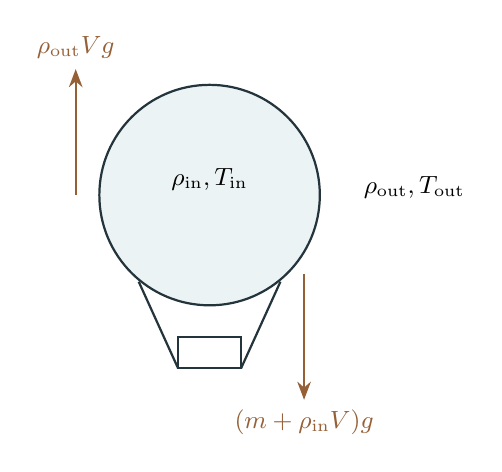
\begin{tikzpicture}[x=1cm,y=1cm]\draw[object,fill=accent!8] (2,2.2) circle(1.4);\draw[object] (1.1,1.1)--(1.6,0);\draw[object] (2.9,1.1)--(2.4,0);\draw[object] (1.6,0) rectangle(2.4,.4);\node at (2,2.4) {$\rho_{\rm in},T_{\rm in}$};\node at (4.6,2.3) {$\rho_{\rm out},T_{\rm out}$};\draw[force] (.3,2.2)--(.3,3.8) node[above]{$\rho_{\rm out}Vg$};\draw[force] (3.2,1.2)--(3.2,-.4) node[below]{$(m+\rho_{\rm in}V)g$};
\end{tikzpicture}\figcaption{解图 热1.9A　外部空气提供浮力，球内热空气与球皮、载荷共同贡献重力。}\end{minipage}\end{center}
\textbf{由临界受力求内气质量。}解图热1.9A的向下力为$(m+\rho_{\rm in}V)g$。升空临界条件
\[\rho_{\rm out}Vg=(300+\rho_{\rm in}V)g\]
给出球内空气质量$M_2=M_1-300=3312.62\,\mathrm{kg}$，约为3.31吨。球内、外成分相同且同压，
\[\frac{T_{\rm in}}{T_{\rm out}}
=\frac{\rho_{\rm out}}{\rho_{\rm in}}
=\frac{M_1}{M_1-m}.\]
\result{T_{\rm in}=300.15\frac{3612.62}{3312.62}
=327.33\,\mathrm K\approx54.2^\circ\mathrm C.}
把临界平衡整理成无量纲形式，更能看清升温承担的作用：
\[\frac m{\rho_{\rm out}V}=1-\frac{\rho_{\rm in}}{\rho_{\rm out}}
=1-\frac{T_{\rm out}}{T_{\rm in}}.\]
本题左边约为0.0830，表示外界空气与球内热空气的密度差约为环境密度的 $8.30\%$。解图热1.9A的浮力仍等于排开外界空气的重量；升温降低的是同体积内部气体的重量。由$T_{\rm in}/T_{\rm out}=1/(1-0.0830)$，温度上升比例约9.06\%，与直接计算一致。

计算成立的条件是$m<\rho_{\rm out}V$，否则即使把内气密度降至趋零，也无法承载。若保留内部压强$p_{\rm in}$略高这一效应，则温度还应乘以$p_{\rm in}/p_{\rm out}$；这里按题意采用同压近似。
\subsubsection*{同成分气体的质量关系与载荷条件}
图热1.9的300千克只包括球皮、吊篮和装载；最大直径给定的是排开外界空气的总体积。
以$\mu$表示空气摩尔质量，两个同体积状态各自满足
\[
p_{\rm in}V=\frac{M_2}{\mu}RT_{\rm in},\qquad
p_{\rm out}V=\frac{M_1}{\mu}RT_{\rm out}.
\]
两式相除，再用解图热1.9A的$M_2=M_1-m$，得
\[
T_{\rm in}=\frac{p_{\rm in}}{p_{\rm out}}
\frac{M_1}{M_1-m}T_{\rm out}.
\]
内、外空气成分相同，摩尔质量 $\mu$ 在比值中约去；质量差由上面的受力平衡给出。
排开的外界空气和球内热空气是不同气体对象，质量之差恰为需要承载的$m$。

按题设忽略微小压差，内气密度为
\[
\rho_{\rm in}=\rho_{\rm out}-\frac mV
\simeq1.08481\,\mathrm{kg/m^3}.
\]
排开外气质量约 3612.62 千克，内气质量约 3312.62 千克。因此 $V(\rho_{\rm out}-\rho_{\rm in})=300$ 千克，正是浮力扣除内气重量后可托起的质量。
小载荷比$\beta=m/(\rho_{\rm out}V)$时，所需温升可展开为
\[
T_{\rm in}-T_{\rm out}
=T_{\rm out}\frac{\beta}{1-\beta}
=T_{\rm out}[\beta+\beta^2+O(\beta^3)].
\]
本题$\beta\simeq0.08304$，一阶估计的温升约24.93开尔文，完整值约27.18开尔文；
载荷相对排开空气质量虽小，二阶及更高修正仍会使温升增加。

这一同压、定体积的密度降低需要气体可由开口或排气装置逸出，
或在准备状态时装入相应较少的气量。
定容密封时，气体质量和体积均保持，升温增加的是内压。近似等压达到所需密度则由前述排气或准备装气实现。

若保留微小超压$p_{\rm in}=(1+\varepsilon)p_{\rm out}$，
在同一载荷、同一体积下，所需温度为同压结果的$1+\varepsilon$倍。
它提高内气的给定温度密度，故为了获得同一密度差需要稍高温度。
按题设的小超压近似取 $\varepsilon=0$。


\Needspace{18\baselineskip}

\pdfbookmark[2]{第 10 题 浮沉子受压下沉的速度关系}{q10}

\section*{第 10 题\quad 浮沉子受压下沉的速度关系}

薄壁圆柱形浮沉子一端封闭、一端开口，开口向下插入密度为$\rho$的液体。液面上方压强为$p_0$时，闭端刚与液面齐平，装置静止。突然将液面上方压强增为$2p_0$。证明下沉深度$x$与速度$v$满足
\[v^2=2gx-\frac{2p_0}{\rho}\ln\left(1+\frac{\rho gx}{2p_0}\right).\]
空气为理想气体，重量可忽略；液体温度均匀，气体压缩按等温过程处理。采用短气柱近似，忽略气柱高度引起的静水压修正，以$\rho gx$表示附加液压；忽略粘滞阻力及液体附加惯性。压强突变后的体积调整很快，取下沉运动开始时$x=0$、$v=0$。

\begin{center}\begin{minipage}{0.96\linewidth}\centering
\begin{tikzpicture}[x=1cm,y=1cm]\fill[accent!7] (-.7,-.4) rectangle(6,3.6);\draw[object] (-.7,3.2)--(6,3.2) node[right]{液面};\draw[object] (1.5,1.4000000000000001)--(1.5,3.2)--(3,3.2)--(3,1.4000000000000001);\fill[white] (1.52,2.3000000000000003) rectangle(2.98,3.18);\node at (2.25,2.75) {$V$};
\node at (4.5,3.8) {$p_0$};\node at (4.3,1.9) {初始悬浮};
\end{tikzpicture}\figcaption{图 热1.10　闭端初始与液面齐平；短气柱近似中取初压为$p_0$。}\end{minipage}\end{center}

\Needspace{8\baselineskip}\subsection*{解答}

\textbf{状态方程给出随深度变化的浮力。}设浮沉子自身质量$M$，初始气体体积$V_0$。按薄壁、短气柱近似，初始静力条件为
\[Mg=\rho gV_0,\qquad M=\rho V_0.\]
加压后的$x=0$处，气体已快速压缩到$V_0/2$，而浮沉子尚无下沉速度。以后闭端下沉$x$，以题目模型中的液压表示气体压强：
\[p(x)=2p_0+\rho gx,\qquad
p_0V_0=(2p_0+\rho gx)V(x).\]
\begin{center}\begin{minipage}{0.96\linewidth}\centering
\begin{tikzpicture}[x=1cm,y=1cm]
\fill[accent!7] (-.35,-.15) rectangle(8.3,3.6);
\draw[guide] (-.35,3.6)--(8.3,3.6);
\foreach \x/\top/\bottom/\ell/\lab in {0/3.6/1.8/.9/{初始$p_0$},2.9/3.6/1.8/.45/{刚加压$2p_0$},5.8/2.3/.5/.3/{下沉后$2p_0$}}{
 \fill[white] (\x+.02,\top-\ell) rectangle(\x+1.48,\top-.02);
 \draw[object] (\x,\bottom)--(\x,\top)--(\x+1.5,\top)--(\x+1.5,\bottom);
 \draw[accent] (\x,\top-\ell)--(\x+1.5,\top-\ell);
 \node[below,align=center,font=\footnotesize] at (\x+.75,-1.1) {\lab};
}
\node at (.75,3.15) {$V_0$};
\node[above,font=\footnotesize] at (3.65,3.67) {$V_0/2$};
\draw[guide] (3.65,3.65)--(3.65,3.4);
\node[right,font=\footnotesize] at (7.4,2.16) {$V(x)<V_0/2$};
\draw[guide] (7.3,2.16)--(7.4,2.16);
\draw[<->] (5.35,2.3)--(5.35,3.6) node[left,midway] {$x$};
\draw[force] (6.55,2.3)--(6.55,2.65) node[above left,font=\footnotesize] {$\rho gV$};
\draw[force] (6.55,.5)--(6.55,-.55) node[below] {$Mg$};
\end{tikzpicture}\figcaption{解图 热1.10A　三状态依次示出气柱缩短；下沉后气压增大，浮力继续减小。}\end{minipage}\end{center}
解图热1.10A的两竖直力给出
\[Mg-\rho gV(x)=Ma,\qquad
a=g\left(1-\frac{V(x)}{V_0}\right)
=g\left(1-\frac{p_0}{2p_0+\rho gx}\right).\]
\textbf{用位置积分求速度。}将加速度写成位置导数，得
\[a=\frac{\dd v}{\dd t}=\frac{\dd v}{\dd x}\frac{\dd x}{\dd t}
=v\frac{\dd v}{\dd x}.\]
两端积分，保留初值$x=0,v=0$：
\begin{align*}
\int_0^v u\dd u
&=g\int_0^x\left(1-\frac{p_0}{2p_0+\rho gs}\right)\dd s\\
\frac{v^2}{2}&=gx-\frac{p_0}{\rho}
\left[\ln\left(1+\frac{\rho gs}{2p_0}\right)\right]_0^x\\
&=gx-\frac{p_0}{\rho}\ln\frac{2p_0+\rho gx}{2p_0}.
\end{align*}
\result{v^2=2gx-\frac{2p_0}{\rho}\ln\left(1+\frac{\rho gx}{2p_0}\right).}
\begin{center}\begin{minipage}{0.96\linewidth}\centering
\begin{tikzpicture}[x=1cm,y=1cm]\draw[axis] (0,0)--(5.8,0) node[right] {$\rho gx/p_0$};\draw[axis] (0,0)--(0,3) node[above] {$a/g$};
\draw[guide] (0,2.5) node[left]{1}--(5.3,2.5);\draw[traj,domain=0:5.2,samples=50] plot (\x,{2.5*(1-1/(2+\x))});\node[left] at (0,1.25) {$1/2$};
\end{tikzpicture}\figcaption{解图 热1.10B　外压突变后初加速度为 $g/2$，随后随下沉深度增大并趋近 $g$。}\end{minipage}\end{center}
\textbf{加速度、速率范围与短气柱近似。}解图热1.10B显示$a(0)=g/2$，对$x>0$有$g/2<a<g$，所以$gx<v^2<2gx$。小深度展开给出
\[v^2=gx+\frac{\rho g^2x^2}{4p_0}+O(x^3),\]
首项与初始加速度$g/2$一致。

有限气柱的气液界面在闭端下方，沿这段高度继续向下，气压式还需加上 $\rho g\ell$。该近似要求气柱高度对应的液压相对于所用绝对压强很小，气体压缩近似等温，且不计液体附加惯性。
\subsubsection*{闭端压差、浮力功与有限气柱的等温压缩}
图热1.10闭端在液面处，而气液界面在闭端下方；
短气柱近似省去的是两点之间的$\rho g\ell$。
按此近似，压强突变后的快速气体调整先使$V_0$变为$V_0/2$，
装置尚来不及产生可计的位移和速度。
解图热1.10A依次画出初始悬浮、刚加压和已经下沉三个状态，
压强增加与下沉都使气体受到进一步压缩，三个状态的气柱长度依次缩短。

以向下为正，运动方程也可写成变力功形式：
\[
\frac{Mv^2}{2}
=\int_0^x[Mg-\rho gV(s)]\,\dd s
=Mgx-\rho g\int_0^x V(s)\,\dd s.
\]
代$M=\rho V_0$及$V(s)=p_0V_0/(2p_0+\rho gs)$，
第二项给出与标准积分相同的对数。
该积分取浮沉子为运动对象，把重力功和随体积改变的浮力功相加。内部气体按等温关系压缩，并通过与周围的热交换维持温度。

对数项在小深度和大深度下分别具有以下极限。令$y=\rho gx/(2p_0)>0$，
由于$0<\ln(1+y)<y$，有$gx<v^2<2gx$。
当$y\to0$，$\ln(1+y)=y-y^2/2+O(y^3)$，
得到已经列出的$v^2=gx+\rho g^2x^2/(4p_0)+O(x^3)$。
当$y\to\infty$，$\ln(1+y)/y\to0$，
所以 $v^2/(2gx)\to1$，从下方趋近自由落体的数值。
在该理想模型中，加速度趋于正的常量$g$，速度随时间继续增大。

有限气柱时，压强应由实际气液界面深度$x+\ell$确定。
设圆柱截面积$S$，初气长$\ell_0$，则
\[
p_{i,\rm gas}=p_0+\rho g\ell_0,\qquad
M=\rho S\ell_0.
\]
后一个关系可由闭端内、外压力差$\rho g\ell_0$乘$S$得到。
压强增加后，令$Q=2p_0+\rho gx$，
等温气体满足
\[
(Q+\rho g\ell)\ell=(p_0+\rho g\ell_0)\ell_0.
\]
先解有限气柱的二次方程求$\ell$，再由$a=g(1-\ell/\ell_0)$积分。
只有$\rho g\ell_0\ll p_0$且运动中$\rho g\ell\ll Q$时，
才退回$p_0V_0=QV$及本题所证的简式。
气柱高度修正进入状态方程；气体按题给等温模型压缩。运动方程中的惯性质量按题意只取浮沉子质量。


\Needspace{18\baselineskip}

\pdfbookmark[2]{第 11 题 由行星大气压强曲线求探测器速度}{q11}

\section*{第 11 题\quad 由行星大气压强曲线求探测器速度}

仪器以恒定速度竖直下降，接近并到达某行星表面，记录压强$p$随时间$t$的曲线（图中压强采用同一约定单位）。到达表面A点时，测得温度$700\,\mathrm K$，重力加速度$10\,\mathrm{m/s^2}$。大气由二氧化碳组成，可视为静止的理想气体，摩尔质量$44\times10^{-3}\,\mathrm{kg/mol}$。由曲线求下降速度。请在图中作A点切线，自行读取所需的压强与时间关系，并说明作图读数对结果精度的限制。

\begin{center}\begin{minipage}{0.96\linewidth}\centering
\begin{tikzpicture}[x=1cm,y=1cm]\draw[axis] (0,0)--(6.2,0) node[right] {$t/\mathrm s$};\draw[axis] (0,0)--(0,3.9) node[above] {$p$/约定单位};

\foreach \x/\v in {1.35/1000,2.7/2000,4.05/3000,5.4/4000}{\draw (\x,0)--(\x,-.07) node[below]{\v};}
\foreach \y/\v in {1.15/20,2.3/40,3.45/60}{\draw (0,\y)--(-.07,\y) node[left]{\v};}
\draw[traj] plot[smooth] coordinates{(0,.015)(1.35,.05)(2.025,.12)(2.7,.32)(3.375,.87)};
\draw[traj] (3.375,.87) .. controls (4,1.45) and (4.35,1.83503) .. (4.86,3.1625);
\fill[accent] (4.86,3.1625) circle(1.5pt);\node[above] at (4.86,3.1625){A};
\end{tikzpicture}\figcaption{图 热1.11　端点 A 对应行星表面。由 A 点的切线读取当地压强变化率。}\end{minipage}\end{center}

\Needspace{8\baselineskip}\subsection*{解答}

\textbf{由静力平衡连接$p,h,t$。}取下降距离$h$向下为正，探测器在$\dd t$内下降$\dd h=v\dd t$。静止大气中的压强增量满足
\[\dd p=\rho g\dd h.\]
\begin{center}\begin{minipage}{0.96\linewidth}\centering
\begin{tikzpicture}[x=1cm,y=1cm]\draw[object] (0,0)--(5.4,0) node[right]{地面};\draw[guide] (0,2.5)--(5.4,2.5);\draw[guide] (0,1.7)--(5.4,1.7);\node[left] at (0,2.5){$p$};\node[left] at (0,1.7){$p+\dd p$};\draw[motion] (2.7,2.5)--(2.7,1.7) node[right,midway]{$\dd h=v\dd t$};\node at (2.7,.7) {$\dd p=\rho g\dd h$};
\end{tikzpicture}\figcaption{解图 热1.11B　$h$取向下的下降距离，因而$\dd p$与$\dd h$同号。}\end{minipage}\end{center}
解图热1.11B把下降距离取为正，因此压强的增量与下降距离的增量同号。由理想气体状态方程$pV=(M/\mu)RT$，得到局部密度
\[\rho=\frac MV=\frac{\mu p}{RT}.\]
代入并使用链式法则：
\[\frac{\dd p}{\dd t}=\rho gv=\frac{\mu pg}{RT}v,\qquad
v=\frac{RT}{\mu g}\frac1p\frac{\dd p}{\dd t}.\]
公式中的 $p,T,g$ 都取仪器当时所在位置的数值。
\begin{center}\begin{minipage}{0.96\linewidth}\centering
\begin{tikzpicture}[x=1cm,y=1cm]\draw[axis] (0,0)--(6.2,0) node[right] {$t/\mathrm s$};\draw[axis] (0,0)--(0,3.9) node[above] {$p$/约定单位};

\foreach \x/\v in {1.35/1000,2.7/2000,4.05/3000,5.4/4000}{\draw (\x,0)--(\x,-.07) node[below]{\v};}
\foreach \y/\v in {1.15/20,2.3/40,3.45/60}{\draw (0,\y)--(-.07,\y) node[left]{\v};}
\draw[traj] plot[smooth] coordinates{(0,.015)(1.35,.05)(2.025,.12)(2.7,.32)(3.375,.87)};
\draw[traj] (3.375,.87) .. controls (4,1.45) and (4.35,1.83503) .. (4.86,3.1625);
\fill[accent] (4.86,3.1625) circle(1.5pt);\node[above] at (4.86,3.1625){A};\draw[guide] (3.645,0)--(4.86,3.1625);\draw[guide] (4.86,0)--(4.86,3.1625);\draw[<->] (3.645,-.65)--(4.86,-.65) node[midway,below]{约900 s};\draw[guide] (0,3.1625) node[left]{55}--(4.86,3.1625);
\end{tikzpicture}\figcaption{解图 热1.11A　切线从零压水平线升至 A 点，升高约55个压强单位，横跨约900 s。}\end{minipage}\end{center}
\textbf{读端点切线。}解图热1.11A中，A点的$p_A\approx55$约定单位；切线从时间轴升到A点，水平跨度约900 s。因此
\[\left(\frac{\dd p}{\dd t}\right)_A\approx\frac{55}{900}
\quad(\text{约定单位}/\mathrm s),\qquad
\frac1{p_A}\left(\frac{\dd p}{\dd t}\right)_A\approx\frac1{900\,\mathrm s}.\]
图中纵轴按绝对压强统一缩放，比例因子在比值中约去。代入$R=8.314\,\mathrm{J/(mol\,K)}$，
\result{v\approx\frac{8.314\times700}{(44\times10^{-3})\times10\times900}
=14.7\,\mathrm{m/s}\approx15\,\mathrm{m/s}.}
约15米每秒的精度取决于可从图上确定的切线方向。整段割线给的是压强关于时间的平均变化率。若改用向上的高度$z$，则$\dd p/\dd z=-\rho g$，$\dd z/\dd t=-v$，两个负号相消，速度大小不变。
\subsubsection*{切线截距为何直接给出局部变化时间}
解图热1.11B中的薄层受力给出的是局部静力关系，
将$\rho=\mu p/(RT)$代入后可写成
\[
\frac{\dd\ln p}{\dd h}=\frac{\mu g}{RT},\qquad
\frac{\dd\ln p}{\dd t}=\frac{\mu g}{RT}v.
\]
取局部极限时，温度与重力加速度按该薄层的数值代入。
若改用向上的几何高度，两式的空间导数符号改变，下降速度的方向也改变，
速度大小仍为正。

令端点坐标为$(t_A,p_A)$，在解图热1.11A中切线与时间轴交于$(t_I,0)$。
切线方程为
\[
p_{\rm tan}(t)=p_A+\dot p_A(t-t_A).
\]
取$p_{\rm tan}(t_I)=0$，便有
\[
\Delta t=t_A-t_I=\frac{p_A}{\dot p_A},\qquad
v_A=\frac{RT_A}{\mu g_A\,\Delta t}.
\]
图上的900秒是把A处压强除以A处变化率得到的局部时间尺度。落地历时由探测器的出发时刻与到达时刻的差给出。

给定端点温度和成分，局部压强标高为
\[
H_p=\frac{RT_A}{\mu g_A}
=\frac{8.314\times700}{0.044\times10}
\,\mathrm m\simeq1.32268\times10^4\,\mathrm m.
\]
于是$v_A=H_p/\Delta t\simeq14.6965\,\mathrm{m/s}$。
切线跨度由图读取，因此结果取约15米每秒。
若近地点一小段还可取$T,g,v$均近似常量，
则$p(t)\simeq p_A\exp[(t-t_A)/\Delta t]$，
这一局部指数函数在A点与观测曲线有同一个函数值和切线斜率。

若压强读数为$u=ap$，同一比例$a$在$\dot u/u$中约去。
若仪表还有零点偏移$u=ap+b$，应改用$\dot u/(u-b)$；
图上读截距时，绝对零压对应 $u=b$；切线与该水平线的交点给出校正后的时间跨度。

读图误差也宜与截距法保持一致。其他量固定时，
\[
\frac{\delta v}{v}\simeq-\frac{\delta(\Delta t)}{\Delta t}.
\]
例如读得$\Delta t=900\pm100$秒，仅由这一读数给出的速度范围约为13.2至16.5米每秒。
同一切线上的压强和斜率读数相关，直接读横向跨度便可一并处理两者的变化。


\Needspace{18\baselineskip}

\pdfbookmark[2]{第 12 题 用体积百分比求标准状态空气密度}{q12}

\section*{第 12 题\quad 用体积百分比求标准状态空气密度}

混合理想气体中某组分的体积百分比，指将该组分单独置于与混合气体相同的温度、压强时，其体积与混合气体总体积之比。空气中氮气、氧气、氩气的体积百分比分别为78\%、21\%、1\%，相对分子质量分别为28.0、32.0、39.9。求标准状态（$1\,\mathrm{atm}$、$0^\circ\mathrm C$）的空气密度。

\begin{center}\begin{minipage}{0.96\linewidth}\centering
\begin{tikzpicture}[x=1cm,y=1cm]\draw[object] (0,0) rectangle(6,1.2);\fill[accent!15] (0,0) rectangle(4.68,1.2);\fill[warm!15] (4.68,0) rectangle(5.94,1.2);\node at (2.34,.6){氮78\%};\node[font=\footnotesize] at (5.28,.6){氧21\%};\draw[guide] (5.97,1.2)--(6.5,1.8) node[right]{氩1\%};\node at (3,-.5){各组分单独置于相同$p,T$时的等效体积};
\end{tikzpicture}\figcaption{图 热1.12　各组分在共同压强和温度下的等效体积给出气体组成，混合后各组分均充满容器。}\end{minipage}\end{center}

\Needspace{8\baselineskip}\subsection*{解答}

\textbf{由定义转成摩尔分数与分压。}取混合气体状态为$p,T,V$。将组分单独置于相同$p,T$时，
\[V_{N_2}=0.78V,\quad V_{O_2}=0.21V,\quad V_{Ar}=0.01V.\]
各组分的$n_i=pV_i/(RT)$，总摩尔数$n=pV/(RT)$，因此$n_i/n=V_i/V=x_i$。故这三项百分数可以直接作为摩尔分数，质量份额另由各组分的摩尔质量得到。
\begin{center}\begin{minipage}{0.96\linewidth}\centering
\begin{tikzpicture}[x=1cm,y=1cm]\draw[object] (0,0) rectangle(2.2,2);\node[align=center] at (1.1,1){组分$i$\\$V_i=x_iV$\\压强$p$};\draw[motion] (2.5,1)--(3.6,1);\draw[object] (4,0) rectangle(7,2);\node[align=center] at (5.5,1){同一组分扩展到$V$\\分压$p_i=x_ip$};\node at (3.5,-.5){温度$T$、摩尔数$n_i$均不变};
\end{tikzpicture}\figcaption{解图 热1.12A　混合后每种气体都占据总体积$V$，其分压与摩尔分数成正比。}\end{minipage}\end{center}
按解图热1.12A，将某组分等温扩展到总体积$V$，摩尔数不变，
\[p_iV=pV_i,\qquad p_i=x_ip.\]
各组分共同占据$V$，并各自贡献分压。故
\[p_{N_2}=0.78p,\quad p_{O_2}=0.21p,\quad p_{Ar}=0.01p.\]
\textbf{方法一：分密度相加。}对于组分$i$，
\[\rho_i=\frac{M_i}{V}=\frac{p_i\mu_i}{RT},\qquad
\rho=\sum_i\rho_i.\]
取$p=101325\,\mathrm{Pa}$、$T=273.15\,\mathrm K$、$R=8.314$，并将摩尔质量换成kg/mol：
\begin{align*}
\rho_{N_2}&=\frac{0.78\times101325\times0.0280}{8.314\times273.15}
\approx0.9744\,\mathrm{kg/m^3},\\
\rho_{O_2}&=\frac{0.21\times101325\times0.0320}{8.314\times273.15}
\approx0.2998\,\mathrm{kg/m^3},\\
\rho_{Ar}&=\frac{0.01\times101325\times0.0399}{8.314\times273.15}
\approx0.01780\,\mathrm{kg/m^3}.
\end{align*}
\Needspace{13\baselineskip}\textbf{方法二：平均摩尔质量。}总质量为$M=\sum n_i\mu_i=n\sum x_i\mu_i$，于是
\[\bar\mu=0.78\times28.0+0.21\times32.0+0.01\times39.9
=28.959\,\mathrm{g/mol}.\]
\result{\rho=\frac{p\bar\mu}{RT}=1.2921\,\mathrm{kg/m^3}\approx1.29\,\mathrm{kg/m^3}.}
把分密度求和时提出公共因子 $p/(RT)$，剩下的正好是平均摩尔质量。总密度用未舍入的各项计算，再按输入的精度报告。
\subsubsection*{分密度与纯气体密度的区别}
图热1.12给出的78、21、1份体积，是各组分分别在共同$p,T$下的等效体积，
混合态中所有组分共同占据总体积 $V$，
其摩尔数$n_i$不变，按解图热1.12A有$p_i=x_ip$。
各组分的摩尔份额满足 $\sum x_i=1$，把分压 $p_i=x_ip$ 相加即得 $\sum p_i=p$。

纯气体密度和分密度用的是两个体积。
设$\rho_i^{(p)}$为组分单独处在总压$p$、温度$T$时的纯气体密度，
而$\rho_i$为该组分在混合气体中的分密度，则
\[
\rho_i^{(p)}=\frac{M_i}{V_i}=\frac{p\mu_i}{RT},\qquad
\rho_i=\frac{M_i}{V}=\frac{p_i\mu_i}{RT}
=x_i\rho_i^{(p)}.
\]
所以总密度既可写成$\sum\rho_i$，也可写成$\sum x_i\rho_i^{(p)}$，
换用总压下的纯气体密度时，每项要乘该组分的体积比例 $x_i$，这一步把分母从 $V_i$ 换成 $V$。

质量份额还需要摩尔质量加权：
\[
w_i=\frac{M_i}{M}=\frac{x_i\mu_i}{\bar\mu},\qquad
\bar\mu=\sum_i x_i\mu_i.
\]
本题得到$w_{N_2}\simeq0.75417$、$w_{O_2}\simeq0.23205$、
$w_{Ar}\simeq0.01378$。氮的78\%体积分数只对应约75.42\%质量；
氩的质量份额约1.38\%，高于其1\%体积份额。
\begin{center}\begin{minipage}{0.96\linewidth}\centering
\begin{tikzpicture}[x=1cm,y=1cm]
\fill[accent!15] (0,1.3) rectangle(4.68,2.2);
\fill[warm!15] (4.68,1.3) rectangle(5.94,2.2);
\fill[gray!25] (5.94,1.3) rectangle(6,2.2);
\draw[object] (0,1.3) rectangle(6,2.2);
\node[left] at (0,1.75) {体积/摩尔};
\node at (2.34,1.75) {氮78\%};\node[font=\footnotesize] at (5.31,1.75) {氧21\%};
\fill[accent!15] (0,0) rectangle(4.52501813,.9);
\fill[warm!15] (4.52501813,0) rectangle(5.9173314,.9);
\fill[gray!25] (5.9173314,0) rectangle(6,.9);
\draw[object] (0,0) rectangle(6,.9);
\node[left] at (0,.45) {质量};
\node at (2.26,.45) {氮75.42\%};\draw[guide] (5.25,0)--(5.25,-.16);
\node[font=\footnotesize,below] at (5.15,-.22) {氧23.21\%};
\draw[guide] (5.97,2.2)--(6.6,2.55) node[right,font=\footnotesize] {氩1\%};
\draw[guide] (5.96,.15)--(6.6,-.3) node[right,font=\footnotesize] {氩1.38\%};
\end{tikzpicture}
\figcaption{解图 热1.12B　同一组成的两种份额；质量条按$x_i\mu_i$重新归一化。}
\end{minipage}\end{center}
图中的两条分别以总摩尔数和总质量为1归一化。同一组分的摩尔数与质量保持，条宽的变化来自归一化所用总量和组分摩尔质量的差别。
若反过来给质量分数，应先求$n_i=Mw_i/\mu_i$，故
\[
x_i=\frac{w_i/\mu_i}{\sum_j w_j/\mu_j},\qquad
\bar\mu=\left(\sum_i\frac{w_i}{\mu_i}\right)^{-1}.
\]
质量分数由总质量归一化，因此得到倒数加权。

最后按未舍入数值相加，三项密度之和约为$1.29208\,\mathrm{kg/m^3}$，
与$101325\times0.028959/(8.314\times273.15)$完全一致。
输入组成和摩尔质量的有效数字有限，报告约$1.29\,\mathrm{kg/m^3}$即可；
上面的分密度小数用于展示各项贡献，总和由未舍入值计算。


\Needspace{18\baselineskip}

\pdfbookmark[2]{第 13 题 干湿空气浮力差导致的称量差异}{q13}

\section*{第 13 题\quad 干湿空气浮力差导致的称量差异}

同一铝片分别在干空气和湿空气中用铜砝码称量。总压均为$760\,\mathrm{mmHg}$、温度均为$20^\circ\mathrm C$，湿空气的水蒸气分压为$15.2\,\mathrm{mmHg}$。天平能察觉的最小称量差为$0.1\,\mathrm{mg}$。求铝片至少应有的质量。铝、铜密度分别为$2.7$、$8.5\,\mathrm{g/cm^3}$；同温下、压强$760\,\mathrm{mmHg}$的干空气和纯水蒸气密度分别为$0.0012$、$0.00075\,\mathrm{g/cm^3}$。

\begin{center}\begin{minipage}{0.96\linewidth}\centering
\begin{tikzpicture}[x=1cm,y=1cm]\draw[object] (0,2.2)--(6,2.2);\draw[object] (3,2.2)--(3,.3);\draw[object] (2.4,.3)--(3,1.3)--(3.6,.3);\draw[object] (.5,2.2)--(.5,.8)--(1.8,.8)--(1.8,2.2);\draw[object] (4.2,2.2)--(4.2,.8)--(5.5,.8)--(5.5,2.2);\draw[object,fill=accent!10] (.65,.8) rectangle(1.65,1.2);\draw[object,fill=warm!25] (4.6,.8) rectangle(5.1,1.45);\node at (1.15,.1){铝片};\node at (4.85,.1){铜砝码};\node at (3,3){同温同总压，改变水汽分压};
\end{tikzpicture}\figcaption{图 热1.13　两盘都受空气浮力；天平比较的是物体的有效重力。}\end{minipage}\end{center}

\Needspace{8\baselineskip}\subsection*{解答}

\textbf{先求干、湿空气的密度差。}同温、同总压下，水汽摩尔分数为$15.2/760=0.02$。所给纯水蒸气密度对应760 mmHg，其在湿空气中的分密度只有$0.02\rho_v$；干气占$0.98$。因此
\[\rho_w=0.98\times0.0012+0.02\times0.00075
=0.001191\,\mathrm{g/cm^3},\]
\[\Delta\rho=\rho_d-\rho_w=0.000009\,\mathrm{g/cm^3}.\]
湿空气比干空气轻。直接用水汽份额与两纯气密度之差求 $\Delta\rho$，保留 $9\times10^{-6}$ 的差值。若先把湿空气密度舍入成0.00119，差值会增大约 $11\%$。
\begin{center}\begin{minipage}{0.96\linewidth}\centering
\begin{tikzpicture}[x=1cm,y=1cm]
\draw[object,fill=accent!10] (0,0) rectangle(2,1);
\draw[object,fill=warm!25] (4,0) rectangle(5.4,1);
\node at (1,.5) {铝};\node at (4.7,.5) {铜};
\draw[force] (.45,1)--(.45,2.2) node[above] {$\rho V_{\rm Al}g$};
\draw[force] (.45,-1)--(.45,0) node[left,midway] {$N_{\rm Al}$};
\draw[force] (1.55,0)--(1.55,-1.15) node[right,midway] {$mg$};
\draw[force] (4.3,1)--(4.3,1.38) node[above] {$\rho V_cg$};
\draw[force] (4.3,-1)--(4.3,0) node[left,midway] {$N_{\rm Cu}$};
\draw[force] (5.1,0)--(5.1,-1.15) node[right,midway] {$m_cg$};
\node at (2.7,-1.75) {等臂天平平衡：$N_{\rm Al}=N_{\rm Cu}$};
\end{tikzpicture}\figcaption{解图 热1.13A　等臂天平平衡时，两盘的支持力相等。图中浮力箭头放大，铝片的浮力较大。}\end{minipage}\end{center}
\textbf{对天平两盘分别修正。}令铝片真实质量为$m$，所需铜砝码质量为$m_c$。解图热1.13A中有效重力相等：
\[mg-\rho\frac m{\rho_{Al}}g
=m_cg-\rho\frac{m_c}{\rho_{Cu}}g.\]
因此在空气密度$\rho$中，天平读数为
\[m_c(\rho)=m\frac{1-\rho/\rho_{Al}}{1-\rho/\rho_{Cu}}.\]
湿空气中所需铜砝码较多。两次读数差精确为
\[\Delta m_c=m_c(\rho_w)-m_c(\rho_d)
=\frac{m\Delta\rho(1/\rho_{Al}-1/\rho_{Cu})}
{(1-\rho_d/\rho_{Cu})(1-\rho_w/\rho_{Cu})}.\]
\Needspace{17\baselineskip}\textbf{由灵敏度求最小质量。}阈值$0.1\,\mathrm{mg}=10^{-4}\,\mathrm g$，令$\Delta m_c$达到它，
\result{m_{\min}=
\frac{10^{-4}(1-0.0012/8.5)(1-0.001191/8.5)}
{9\times10^{-6}(1/2.7-1/8.5)}\,\mathrm g
=43.95\,\mathrm g\approx44\,\mathrm g.}
也可用体积差作一阶估算：1 g铝与约1 g铜的体积差为
\[\frac1{2.7}-\frac1{8.5}=0.25272\,\mathrm{cm^3},\]
由此每克样品的称量差约$9\times10^{-6}\times0.25272=2.2745\times10^{-6}$ g；阈值除以该数得到43.97 g，与精确式一致。这个估算使用的是铝与铜的体积差。
\subsubsection*{两盘支持力与读数变化方向}
图热1.13的理想等臂天平比较两盘传来的支持力。
解图热1.13A在铝和铜上各画出重力、浮力及盘的支持力，
静止时分别为
\[
N_{\rm Al}=mg-\rho V_{\rm Al}g,\qquad
N_{\rm Cu}=m_cg-\rho V_cg.
\]
两盘平衡要求$N_{\rm Al}=N_{\rm Cu}$，这才得到正文的砝码读数函数。

这里把对称盘架的自重和浮力视为已调平且两侧相消，比较的是样品与砝码增加的部分。

由精确函数求导，可直接判断符号：
\[
\frac{\dd m_c}{\dd\rho}
=m\frac{1/\rho_{Cu}-1/\rho_{Al}}
{(1-\rho/\rho_{Cu})^2}<0.
\]
空气变湿时$\rho$减小，所需$m_c$反而增加。
因为铝的单位质量体积较大，铝侧损失的浮力比铜侧更多，需增加砝码来重新平衡。
若样品与砝码密度相同，上式恒为零，气体密度变化不产生这种差别。

湿度带来的密度差由分压线性叠加决定：
\[
\Delta\rho=\frac{p_v}{p}(\rho_d-\rho_v)
=0.02(0.0012-0.00075)
=9.0\times10^{-6}\,\mathrm{g/cm^3}.
\]
给定的$\rho_v$是在总压$p$下的纯组分理想气体密度，
实际湿空气中水汽只贡献$(p_v/p)\rho_v$。
按第12题的分密度定义，分别用0.02与0.98乘纯水汽和干气密度，再相加。

精确两次读数差中的分母约为0.999719，若只忽略这个近1的修正，
所得最小质量43.97克与精确43.95克仅差约0.03\%。
若把 $\Delta\rho$ 先舍入为 $10^{-5}\,\mathrm{g/cm^3}$，代入公式的密度差就会增大约 $11.1\%$，
算出的阈值会降至约39.6克；这项舍入影响远大于是否保留砝码浮力分母。
因此小差值应先由未舍入数据求出，再决定哪些高阶修正可忽略。


\Needspace{18\baselineskip}

\pdfbookmark[2]{第 14 题 干空气与湿空气隔板平衡及混合压强}{q14}

\section*{第 14 题\quad 干空气与湿空气隔板平衡及混合压强}

导热长方体容器用不漏气隔板分成两室，分别装有相等质量的干空气和湿空气；湿空气中水蒸气质量占2\%。取干空气、水蒸气摩尔质量分别为$28.8$、$18.0\,\mathrm{g/mol}$。两室与环境等温，不发生凝结。
\begin{enumerate}
\item 隔板可沿器壁自由无摩擦地滑动，求平衡后干空气、湿空气体积比。
\item 另从两室初始体积相等的状态开始，抽出隔板而不漏气，求最终压强与初始干空气压强、湿空气压强三者之比。
\end{enumerate}

\begin{center}\begin{minipage}{0.96\linewidth}\centering
\begin{tikzpicture}[x=1cm,y=1cm]\draw[object] (0,0) rectangle(6,2);\draw[object,line width=1.2pt] (3,0)--(3,2);\node[align=center,text width=2.7cm,font=\footnotesize] at (1.5,1){干空气\quad$M$};\node[align=center,text width=2.7cm,font=\footnotesize] at (4.5,1){湿空气\quad$M$\\干气$0.98M$\\水汽$0.02M$};
\end{tikzpicture}\figcaption{图 热1.14　同质量不等于同摩尔数；两问分别采用可动隔板和初始等体积抽板条件。}\end{minipage}\end{center}

\Needspace{8\baselineskip}\subsection*{解答}

\textbf{先建立摩尔数表。}两室总质量均为$M$；湿空气中的干气、水汽质量为$0.98M$、$0.02M$，因此
\[n_d=\frac M{\mu_a},\qquad
n_w=\frac{0.98M}{\mu_a}+\frac{0.02M}{\mu_v}.\]
由$\mu_a/\mu_v=28.8/18=1.6$得
\[\frac{n_w}{n_d}=0.98+0.02\times1.6=1.012.\]
水汽分子较轻，相等质量的湿空气含更多粒子。

\textbf{（1）可动隔板。}解图热1.14A中平衡时同温、同压：
\[pV_d=n_dRT,\qquad
pV_w=(p_{a,w}+p_{v,w})V_w=n_wRT.\]
将摩尔数代入也可直接写成
\[pV_w=\left(\frac{0.98}{\mu_a}+\frac{0.02}{\mu_v}\right)MRT.\]
\result{V_d:V_w=n_d:n_w=1:1.012,\qquad V_d/V_w\approx0.98814.}
\begin{center}\begin{minipage}{0.96\linewidth}\centering
\begin{tikzpicture}[x=1cm,y=1cm]\draw[object] (0,0) rectangle(6,2);\draw[object,line width=1.2pt] (2.982,0)--(2.982,2);\node[align=center,text width=2.7cm,font=\footnotesize] at (1.5,1){干空气\quad$M$};\node[align=center,text width=2.7cm,font=\footnotesize] at (4.5,1){湿空气\quad$M$\\干气$0.98M$\\水汽$0.02M$};\draw[<->] (2.6,2.5)--(3.4,2.5);\node at (1.5,-.45){$V_d\propto n_d$};\node at (4.5,-.45){$V_w\propto n_w$};\node at (3,3.15){可动平衡：同$p$、同$T$};
\end{tikzpicture}\figcaption{解图 热1.14A　湿空气摩尔数稍多，平衡体积稍大；差异仅1.2\%，图中隔板位移很小。}\end{minipage}\end{center}
\textbf{（2）初始等体积，抽板混合。}解图热1.14B从两室各占 $V_0$ 的初态开始，抽板前两侧各有自己的压强。初始
\[p_dV_0=\frac M{\mu_a}RT,\quad
p_wV_0=\left(\frac{0.98M}{\mu_a}+\frac{0.02M}{\mu_v}\right)RT.\]
混合后，干气总质量为$1.98M$、水汽总质量为$0.02M$，总体积$2V_0$。因此
\[p_f(2V_0)=\left(\frac{1.98M}{\mu_a}+\frac{0.02M}{\mu_v}\right)RT
=(p_d+p_w)V_0.\]
\begin{center}\begin{minipage}{0.96\linewidth}\centering
\begin{tikzpicture}[x=1cm,y=1cm]\draw[object] (0,0) rectangle(6,2);\draw[guide] (3,0)--(3,2);\draw[motion] (3,2.1)--(3,2.8) node[above]{抽板};\node at (1.5,1){初始$V_0$};\node at (4.5,1){初始$V_0$};\node at (3,-.55){混合后共占$2V_0$，$p_f=(p_d+p_w)/2$};
\end{tikzpicture}\figcaption{解图 热1.14B　第二问从初始等体积状态开始，混合后所有组分共享总体积。}\end{minipage}\end{center}
\result{p_f:p_d:p_w=\frac{1+1.012}{2}:1:1.012
=1.006:1:1.012.}
一般初体积 $V_d,V_w$ 下，终压是按初体积加权的平均压强 $p_f=(p_dV_d+p_wV_w)/(V_d+V_w)$，各项按全程气相摩尔数保持计算。若有凝结，则按剩余气相气量列式。
\subsubsection*{质量分数、分压与混合后的组成}
图热1.14的 $2\%$ 是水汽质量占湿气总质量的份额，先按各自摩尔质量换算为摩尔数。
以干气摩尔数$n_d=M/\mu_a$为单位，湿室的干气、水汽分别有
\[
n_{a,w}=0.98n_d,\qquad
n_{v,w}=0.02\frac{\mu_a}{\mu_v}n_d=0.032n_d.
\]
总摩尔数为$1.012n_d$，水汽在湿气中的摩尔分数及分压比是
\[
x_{v,w}=\frac{0.032}{1.012}\simeq0.03162,
\qquad p_{v,w}=x_{v,w}p_w.
\]
湿气平均摩尔质量为$\mu_w=\mu_a/1.012\simeq28.4585$克每摩尔。
相等质量的湿气摩尔数较多，因此温度和压强相同时，湿室体积较大。

解图热1.14A的隔板只略向干室移动。
若初始等分总体积$2V_0$，平衡体积为
\[
V_d=\frac{2V_0}{2.012},\qquad
V_w=\frac{2\times1.012V_0}{2.012}.
\]
湿室体积比干室大1.2\%，但隔板相对于中线的位移只占容器全长的
\[
\frac12-\frac1{2.012}\simeq0.002982.
\]
因此图中把全长画为6厘米时，干室宽约2.98211厘米，位移约0.01789厘米。
体积比的1.2\%与全长位移百分数使用不同的分母。

第二问重新从等体积初态抽板。设初始干室压强为$p_d$，
湿室的两个分压为$0.98p_d$和$0.032p_d$。
解图热1.14B中每种组分最后都占$2V_0$，所以最终
\[
p_{a,f}=\frac{1+0.98}{2}p_d=0.99p_d,\qquad
p_{v,f}=\frac{0.032}{2}p_d=0.016p_d.
\]
相加即得$p_f=1.006p_d$。最终水汽质量只占总质量的1\%，
其摩尔分数为
\[
x_{v,f}=\frac{0.032}{2.012}\simeq0.01590.
\]
质量份额与摩尔份额都应以混合后的新总量归一化。
若初始水汽未饱和且全程同温、没有另加水，第二问水汽分压降低一半，
因而不会仅由这次等温扩展新产生凝结。

若从第一问已经同温同压的可动平衡状态抽板，
两室原有$pV_d=n_dRT$、$pV_w=n_wRT$，
相加后仍是$p(V_d+V_w)=(n_d+n_w)RT$，
故混合后压强仍为$p$。
解图热1.14A给出可动隔板的同压状态。解图热1.14B的抽板则从两室等体积时开始。


\Needspace{18\baselineskip}

\pdfbookmark[2]{第 15 题 潮湿空气压缩凝结与降温后的压强}{q15}

\section*{第 15 题\quad 潮湿空气压缩凝结与降温后的压强}

均匀导热长圆管下端封闭、上端开口，竖直放置。初始$27^\circ\mathrm C$、$760\,\mathrm{mmHg}$、相对湿度75\%的空气充满全管，管口用无摩擦、质量可忽略的薄活塞封住。$27^\circ\mathrm C$、$0^\circ\mathrm C$的饱和水蒸气压分别为$26.7$、$4.58\,\mathrm{mmHg}$。
\begin{enumerate}
\item 等温地向活塞上方注入水银，使管内开始出现水珠，管至少须多长？
\item 水蒸气刚开始凝结时固定活塞，再降温至$0^\circ\mathrm C$，求管内总压强。
\end{enumerate}
忽略凝结水所占体积、活塞厚度及热膨胀；相对湿度为实际水汽分压与同温饱和压之比。

\begin{center}\begin{minipage}{0.96\linewidth}\centering
\begin{tikzpicture}[x=1cm,y=1cm]
\fill[accent!8] (0,0) rectangle(2,3);
\draw[object] (0,3)--(0,0)--(2,0)--(2,3);
\draw[object,line width=2pt] (0,3)--(2,3);
\node[align=center] at (1,1.5) {湿空气\\$L_0$};
\node[above] at (1,3.15) {$p_0$};
\node[align=left] at (4.4,2.4) {$\varphi=75\%$\\$T=27^\circ\mathrm C$};
\draw[motion] (3.3,.8)--(3.3,1.8) node[right,midway] {加汞增压};
\end{tikzpicture}\figcaption{图 热1.15　等温压缩前两种气体分压都按固定摩尔数变化。}\end{minipage}\end{center}

\Needspace{8\baselineskip}\subsection*{解答}

\textbf{（1）压缩到刚饱和。}初始水汽分压由相对湿度定义给出
\[p_{v0}=0.75\times26.7=20.025\,\mathrm{mmHg}.\]
在出现凝结前，水汽与干气摩尔数各自不变。设饱和时气长为$L$，水汽的等温关系为
\[p_{v0}L_0=p_s(27^\circ\mathrm C)L,\qquad L=0.75L_0.\]
全部气体也在这段压缩中守恒，因此总压
\[p_1=p_0\frac{L_0}{L}=\frac{760}{0.75}
=1013.333\,\mathrm{mmHg}.\]
\begin{center}\begin{minipage}{0.96\linewidth}\centering
\begin{tikzpicture}[x=1cm,y=1cm]
\fill[accent!8] (0,0) rectangle(2,2.25);
\fill[warm!35] (0,2.25) rectangle(2,3);
\draw[object] (0,3)--(0,0)--(2,0)--(2,3);
\draw[object,line width=2pt] (0,2.25)--(2,2.25);
\node[align=center] at (1,1.1) {气体\\$L=.75L_0$};
\node at (1,2.625) {汞：$h$};
\draw[<->] (2.5,2.25)--(2.5,3) node[right,midway] {$h\le.25L_0$};
\node[align=center] at (6.1,2.6) {$p_v=p_s(27^\circ\mathrm C)$\\固定活塞，再降温};
\draw[motion] (6.1,1.9)--(6.1,1);
\node[align=center] at (6.1,.45) {干气气量固定\\水在气液间重新分配};
\end{tikzpicture}\figcaption{解图 热1.15A\quad 刚饱和时气柱长$0.75L_0$，活塞上方只剩$0.25L_0$容纳水银。}\end{minipage}\end{center}
解图热1.15A显示，活塞上方的空隙只有$L_0-L=0.25L_0$。质量可忽略的活塞需由水银提供附加压强：所需汞高
\[h=p_1-p_0=253.333\,\mathrm{mm},\]
压强差用毫米汞柱表示，汞柱的几何高度用毫米表示，两者数值相同。能容下此水银的条件为
\[0.25L_0\ge253.333\,\mathrm{mm}.\]
\result{L_0\ge1013.333\,\mathrm{mm}\approx1.013\,\mathrm m.}
管长恰取临界值时，管内刚好饱和，汞面也恰到管口。若要继续靠等温加汞压出水珠，管长应稍大于这个值，为附加的汞柱留出空间。
\begin{center}\begin{minipage}{0.96\linewidth}\centering
\begin{tikzpicture}[x=1cm,y=1cm]\draw[axis] (0,0)--(5.4,0) node[right] {$V_0/V$};\draw[axis] (0,0)--(0,3.5) node[above] {$p_v/\mathrm{mmHg}$};
\draw[guide] (0,2.67) node[left]{26.7}--(5,2.67);\draw[traj] (2,2.0025)--(2.6667,2.67)--(5,2.67);\draw[guide] (2,0) node[below]{1}--(2,2.0025)--(0,2.0025) node[left]{20.025};\draw[guide] (2.6667,0) node[below]{$4/3$}--(2.6667,2.67);\node at (4.3,1.2){凝结区};
\end{tikzpicture}\figcaption{解图 热1.15B　等温压缩先使水汽分压升高。达到饱和后继续压缩，部分水汽凝结，分压保持饱和值。}\end{minipage}\end{center}
\textbf{（2）固定活塞后降温。}刚饱和时干气分压为
\[p_{a1}=p_1-26.7=986.6333\,\mathrm{mmHg}.\]
干气摩尔数、体积保持不变，由$p_a/T=\text{常量}$，
\[p_{af}=986.6333\frac{273.15}{300.15}
=897.8807\,\mathrm{mmHg}.\]
水汽若不凝结，本来会达到$26.7\times273.15/300.15=24.30\,\mathrm{mmHg}$，高于0℃的饱和压4.58 mmHg，气相减少到与液滴平衡时的饱和分压。
\result{p_f=p_{af}+p_{vf}=897.8807+4.58
=902.4607\,\mathrm{mmHg}\approx902.5\,\mathrm{mmHg}.}
气相水汽的摩尔数比例为
\[\frac{n_{vf}}{n_{v1}}=\frac{p_{vf}/T_f}{p_{v1}/T_1}
=\frac{4.58\times300.15}{26.7\times273.15}\approx0.1885.\]
其余约81.2\%已经凝结。解图热1.15B的水平段说明饱和后的水汽压强由温度决定；凝结量由总水量减去饱和水汽量得到。
\subsubsection*{临界长度的容量限制与固定活塞的作用}
图热1.15的初始活塞在管口，气体占据全长$L_0$。
解图热1.15A将活塞厚度作为零厚度粗线，气柱长与活塞上方空隙的交界就是该粗线的位置。
达到刚饱和时，气柱和可用汞柱空间分别为$0.75L_0$、$0.25L_0$；
最短容器恰能在这两个空间内同时满足饱和条件和活塞受力。
水汽分压26.7毫米汞柱只是总压的一部分，提供活塞负载的汞高须由总压差253.333毫米汞柱确定。

对一般初相对湿度$0<\varphi<1$，同样的步骤给
\[
L=\varphi L_0,\qquad
p_1=\frac{p_0}{\varphi},\qquad
h=P_0\left(\frac1\varphi-1\right),
\]
其中$P_0$是将大气压强表示成汞柱几何高度的数值。
容量要求$(1-\varphi)L_0\ge h$，因$1-\varphi>0$才可约去，得
\[
L_{0,\min}=\frac{P_0}{\varphi}.
\]
$\varphi=1$ 时初态已饱和；若再靠加汞压缩相对体积 $\delta>0$，饱和水汽压保持，气体总压的增量仅来自干气。以 $P_{a0}$ 表示初始干气分压对应的汞高，所需汞高为 $P_{a0}\delta/(1-\delta)$，而空隙为 $\delta L_0$，故 $L_0\ge P_{a0}/(1-\delta)$。$\varphi=0$ 时初始水量为零，等温压缩只改变干气压强。
本题$\varphi=0.75$，才可使用已经求得的1.013米临界长度。

解图热1.15B的水平支是固定温度下水汽的相平衡关系。
要沿这一相平衡支继续压缩，还要用该状态的总压求所需汞高，并与活塞上方的余量比较。
等号给出刚饱和的管长下限。容汞空间允许继续压缩时，形成的液态水量由新体积中饱和水汽的摩尔数决定。

固定活塞后，解图热1.15C中的气柱体积保持$0.75V_0$，
干气摩尔数不变，但水在气相与液相间重新分配。
总水量守恒应写成
\[
n_{v1}=n_{vf}+n_{\ell f},\qquad
n_{vf}=\frac{p_s(T_f)V}{RT_f}.
\]
用同体积下两温度的 $p_v/T$ 求气相份额，其余水量计为液相。
若液体体积可略，任意终温时水汽压的一般选择为
\[
p_{vf}=\min\left[p_{v1}\frac{T_f}{T_1},p_s(T_f)\right].
\]
取其中较小的分压，与定量、定容的干气压相加。

若活塞上方的汞负载保持，外侧压力仍为$p_1$；
降温后内部总压约902.4607毫米汞柱，低于该外压。
活塞锁定装置需提供向上的支持，大小为
\[
\frac{F_{\rm lock}}S=p_1-p_f
\simeq110.8726\,\mathrm{mmHg}.
\]
解图热1.15C 中，锁定装置提供向上的支持，气体降温时体积保持不变。若活塞可以自由移动，降温后应由外压与气体状态方程重新确定气柱体积。
\begin{center}\begin{minipage}{0.96\linewidth}\centering
\begin{tikzpicture}[x=1cm,y=1cm]
\foreach \x/\temp/\pa/\pv in {0/{27^\circ\mathrm C}/{986.6333}/{26.7},4.3/{0^\circ\mathrm C}/{897.8807}/{4.58}}{
 \fill[accent!8] (\x,0) rectangle(\x+2.5,2.1);
 \draw[object] (\x,2.1)--(\x,0)--(\x+2.5,0)--(\x+2.5,2.1);
 \draw[object,line width=2pt] (\x,2.1)--(\x+2.5,2.1);
 \draw[object] (\x-.2,2.1)--(\x+.15,2.1);
 \draw[object] (\x+2.35,2.1)--(\x+2.7,2.1);
 \node[above] at (\x+1.25,2.25) {$\temp$};
 \node[align=center,font=\footnotesize] at (\x+1.25,1.25) {$p_a=\pa$\\$p_v=\pv$\\单位：mmHg};
 \node[below] at (\x+1.25,0) {活塞固定，$V=.75V_0$};
}
\foreach \x in {4.6,5.05,5.5,5.95,6.4}{\fill[accent!65] (\x,.12) circle(1.7pt);}
\draw[motion] (2.9,1.1)--(3.9,1.1) node[midway,above,font=\footnotesize] {降温};
\draw[force] (7.3,1.1)--(7.3,2.1) node[right,midway] {$F_{\rm lock}$};
\end{tikzpicture}
\figcaption{解图 热1.15C　干气分压按温度降低，水汽凝结；锁定支持维持相同气体体积。}
\end{minipage}\end{center}


\Needspace{18\baselineskip}

\pdfbookmark[2]{第 16 题 可分解双原子气体升温后的水银柱移动}{q16}



\section*{第 16 题\quad 可分解双原子气体升温后的水银柱移动}

两端封闭的均匀石英管竖直放置，中间水银柱将下方空气和上方可分解双原子气体隔开。初始温度$T_0$，下、上气柱长分别为$2l_0$、$l_0$。水银柱重力对应的压强为下方初始压强$p_0$的$\alpha$倍（$0<\alpha<1$）。温度超过$T_0$后，上方有$\Delta n$个双原子分子分解为$2\Delta n$个单原子粒子；小温升满足
\[\frac{\Delta n}{n_0}=\frac{\Delta T}{T_0}=\varepsilon\ll1,\]
其中$n_0$为初始双原子分子数。上下气体温升相同，忽略管和水银热膨胀。判断水银柱上升还是下降，并说明临界情形。

\begin{center}\begin{minipage}{0.96\linewidth}\centering
\begin{tikzpicture}[x=1cm,y=1cm]\fill[accent!8] (0, 0) rectangle (2,2);
\node[align=center,font=\footnotesize] at (1.0,1.0) {空气\\$2l_0,p_0$};
\fill[warm!35] (0, 2) rectangle (2,2.5);
\node[align=center,font=\footnotesize] at (1.0,2.25) {汞};
\fill[accent!8] (0, 2.5) rectangle (2,3.5);
\node[align=center,font=\footnotesize] at (1.0,3.0) {双原子气\\$l_0$};
\draw[object] (0,0)--(0,3.5);\draw[object] (2,0)--(2,3.5);
\draw[object] (0,0)--(2,0);
\draw[object] (0,3.5)--(2,3.5);
\node[align=center] at (1.0,-.55) {初始$T_0$};
\node[align=center] at (5,2.2){水银重力/截面积\\$=\alpha p_0$};
\end{tikzpicture}\figcaption{图 热1.16　初始上方压强为$(1-\alpha)p_0$；上方分解会改变粒子总数。}\end{minipage}\end{center}

\Needspace{8\baselineskip}\subsection*{解答}

\textbf{固定水银位置作虚拟比较。}初态下方压强为$p_0$，上方为$(1-\alpha)p_0$，压强差平衡汞柱重力。先暂设体积不变，则下方空气升温后
\[p_1=p_0(1+\varepsilon).\]
上方原有摩尔数$\nu_0$。分解后未分解双原子气和新生单原子气分别为
\[\nu_{\text{双}}=\nu_0(1-\varepsilon),\qquad
\nu_{\text{单}}=2\nu_0\varepsilon,\]
总摩尔数为$\nu_0(1+\varepsilon)$，每分解一个旧粒子得到两个新粒子，因此净增加 $\nu_0\varepsilon$。
\begin{center}\begin{minipage}{0.96\linewidth}\centering
\begin{tikzpicture}[x=1cm,y=1cm]
\fill[accent!8] (0,0) rectangle(1.6,2);
\fill[warm!35] (0,2) rectangle(1.6,2.5);
\fill[accent!8] (0,2.5) rectangle(1.6,3.5);
\draw[object] (0,0) rectangle(1.6,3.5);
\node at (.8,1) {下：$p_1$};\node at (.8,2.25) {汞};\node at (.8,3) {上：$p_2$};
\node[below] at (.8,-.2) {虚设汞不动};
\draw[object,fill=warm!35] (3.2,2) rectangle(4.8,2.5);
\draw[force] (3.55,1)--(3.55,2) node[left,midway] {$p_1S$};
\draw[force] (3.55,3.5)--(3.55,2.5) node[left,midway] {$p_2S$};
\draw[force] (4.4,2.25)--(4.4,1.1) node[right,midway] {$\alpha p_0S$};
\node[align=left,font=\footnotesize] at (6.7,2.8) {$n_0-\Delta n$个双原子\\$2\Delta n$个单原子\\总数$n_0+\Delta n$};
\end{tikzpicture}\figcaption{解图 热1.16A　在初始位置分别画向上的下气压力、向下的上气压力与汞重。箭头表示各力的方向。}\end{minipage}\end{center}
\textbf{分压相加得到上方总压。}截面积记为$S$，虚设不动时上方体积仍为$l_0S$：
\begin{align*}
p_{\text{双}}l_0S&=\nu_0(1-\varepsilon)R T_0(1+\varepsilon),\\
p_{\text{单}}l_0S&=2\nu_0\varepsilon R T_0(1+\varepsilon),\\
(1-\alpha)p_0l_0S&=\nu_0RT_0.
\end{align*}
把前两式相加并除以初态式，
\[p_2=(1-\alpha)p_0(1+\varepsilon)^2.\]
解图热1.16A的向下压力为$(p_2+\alpha p_0)S$，向上为$p_1S$。令向下净压差
\begin{align*}
\Delta p&=p_2+\alpha p_0-p_1\\
&=p_0\bigl[(1-2\alpha)\varepsilon+(1-\alpha)\varepsilon^2\bigr]\\
&=p_0\varepsilon\bigl[1+\varepsilon-(2+\varepsilon)\alpha\bigr].
\end{align*}
在题给分解律作为模型等式时，临界值为
\result{\alpha_c=\frac{1+\varepsilon}{2+\varepsilon};\quad
\alpha<\alpha_c:\text{下降},\quad
\alpha>\alpha_c:\text{上升}.}
等于$\alpha_c$时在原位置平衡。对于固定$\alpha$、充分小的正温升，一阶判据为$\alpha<1/2$下降、$\alpha>1/2$上升。$\alpha=1/2$时一阶项为零，按模型等式保留二阶得$\Delta p=p_0\varepsilon^2/2>0$，故微量下降。若分解律是仅到一阶的近似，$\alpha=1/2$ 时应按实际分解律的二阶系数判断，计算见下文。

\textbf{由水银位移求两侧气体压强的变化。}取水银上移$\delta$为正，空气体积变为$S(2l_0+\delta)$，上气体积为$S(l_0-\delta)$。平衡式为
\[\frac{p_0(1+\varepsilon)}{1+\delta/(2l_0)}
-\frac{(1-\alpha)p_0(1+\varepsilon)^2}{1-\delta/l_0}
=\alpha p_0.\]
一阶展开后，
\[(2\alpha-1)\varepsilon-(3/2-\alpha)\frac{\delta}{l_0}=0,
\quad \frac{\delta}{l_0}=\frac{2\alpha-1}{3/2-\alpha}\varepsilon+O(\varepsilon^2).\]
分母始终为正，位移的符号由$2\alpha-1$决定。这个式子同时给出水银移动的方向和一阶位移量；两侧体积的变化又分别决定相应的压强变化。
\subsubsection*{平衡位置的唯一性与小温升展开}
图热1.16与解图热1.16A中的上下两份气体始终由汞隔离；
上方的粒子数由上方气体自身的解离改变。
虚设汞不动只用于计算初始净压力，随后用解图热1.16B中的两段气长表示实际位置的净压力。

以解图热1.16B的$s=\delta/l_0$记向上位移，
正气长要求$-2<s<1$。将向上净压力除$p_0S$，记为
\[
F(s)=\frac{1+\varepsilon}{1+s/2}
-\frac{(1-\alpha)(1+\varepsilon)^2}{1-s}-\alpha.
\]
在题给分解率只随温度规定的模型中，
\[
F'(s)=-\frac{1+\varepsilon}{2(1+s/2)^2}
-\frac{(1-\alpha)(1+\varepsilon)^2}{(1-s)^2}<0.
\]
且$s\to-2^+$时$F\to+\infty$，$s\to1^-$时$F\to-\infty$，
所以每个允许的小温升有唯一的正气长平衡。
$F(0)=-\Delta p/p_0$，因$F$递减，虚设位置的向下净压差为正时，
平衡根必为负位移。相反的初始净压差则给出正位移。净压差随位移减小，偏离新平衡点时，净力指回平衡点。

还可完整展开位移方程而不先丢掉二阶项：
\[
\alpha s^2+B_\delta s+C_\delta=0,
\]
\[
B_\delta=(2\alpha-3)+(2\alpha-4)\varepsilon
+(\alpha-1)\varepsilon^2,\qquad
C_\delta=2\varepsilon[(2\alpha-1)+(\alpha-1)\varepsilon].
\]
与$s=0$初态连续相连的根可写为
\[
s=\frac{2C_\delta}
{-B_\delta+\sqrt{B_\delta^2-4\alpha C_\delta}}.
\]
这一写法由求根式有理化得到，减小了两个相近正数相减时的相消误差。由上下气柱长度均为正，位移范围为 $-2<s<1$。
取一阶即回到正文的$s=(2\alpha-1)\varepsilon/(3/2-\alpha)$；
取$\alpha=1/2$再展开则得
\[
\frac{\delta}{l_0}=-\frac12\varepsilon^2+O(\varepsilon^3),
\]
由负的二阶项得汞柱微量下降。

将临界值按温升展开，得
\[
\alpha_c=\frac{1+\varepsilon}{2+\varepsilon}
=\frac12+\frac14\varepsilon-\frac18\varepsilon^2+O(\varepsilon^3).
\]
当 $\alpha-1/2$ 为 $O(\varepsilon)$ 时，一阶与二阶贡献同阶，直接把 $\alpha$ 与 $\alpha_c$ 比较。
例如$\varepsilon=0.02$时$\alpha_c\simeq0.5049505$，
取$\alpha=0.502$虽然大于1/2，模型仍给下降。

若给出的分解关系只准确到一阶，写成
$f=\Delta n/n_0=\varepsilon+c\varepsilon^2+O(\varepsilon^3)$，
在$\alpha=1/2$时净向下压差改为
\[
\frac{\Delta p}{p_0}
=\frac{1+c}{2}\varepsilon^2+O(\varepsilon^3).
\]
$c>-1$ 时给二阶下降，$c<-1$ 时给二阶上升；$c=-1$ 时再由下一阶系数决定。
固定$\alpha\ne1/2$且温升充分小时，一阶方向判据仍成立。
\begin{center}\begin{minipage}{0.96\linewidth}\centering
\begin{tikzpicture}[x=1cm,y=1cm]
\fill[accent!8] (0,0) rectangle(2,2.25);
\fill[warm!35] (0,2.25) rectangle(2,2.75);
\fill[accent!8] (0,2.75) rectangle(2,3.5);
\draw[object] (0,0) rectangle(2,3.5);
\draw[guide] (-.2,2)--(2.9,2);\draw[guide] (-.2,2.5)--(2.2,2.5);
\node at (1,1) {$2l_0+\delta$};
\node[font=\footnotesize] at (1,3.1) {$l_0-\delta$};
\draw[<->] (2.5,2)--(2.5,2.25) node[right,midway] {$\delta$};
\node[align=left] at (5.5,2.65) {取向上位移为正\\两段气柱总长为 $3l_0$};
\node[align=left] at (5.5,1.25) {$-2<\delta/l_0<1$\\实际正负由压力平衡求出};
\end{tikzpicture}
\figcaption{解图 热1.16B　正位移的几何定义；下气柱加长，上气柱缩短，汞长保持。}
\end{minipage}\end{center}



\end{document}
